\documentclass{memoir}

\usepackage{amsthm,amssymb,amsmath}
\usepackage{makeidx}
\usepackage{xifthen}
\usepackage[inline]{enumitem}
\usepackage{tikz}
  \usetikzlibrary{patterns}
  \usetikzlibrary{cd}
  \usetikzlibrary{calc}
  \usetikzlibrary{arrows}
\usepackage[framemethod=tikz,usetwoside]{mdframed}
\usepackage{hyperref}
  \hypersetup{linktocpage,colorlinks,linkcolor=blue}
\usepackage[figurewithin=section]{caption}
\usepackage{collect}
\usepackage{wasysym}
\usepackage{mathtools}

% #Counters
%

%-----------%
% #Counters %
%-----------%

% Number chapters as I, II, III, etc.
\renewcommand{\thechapter}{\Roman{chapter}}

% Number sections sequentially (not within chapters)
\counterwithout{section}{chapter}

% Number figures and tables within sections
\makeatletter                        %&%
  \renewcommand\@memmain@floats{     %&%
    \counterwithout{figure}{chapter} %&%
    \counterwithin{figure}{section}  %&%
    \counterwithout{table}{chapter}  %&%
    \counterwithin{table}{section}   %&%
  }                                  %&%
\makeatother                         %&%




%%%


% Keep chapter numbers and titles from overlapping in TOC
\renewcommand{\chapternumberlinebox}[2]{\makebox[1cm][l]{#2}}

% Roman-enumerated lists for propositions and proofs
\newenvironment{proplist}[0] %&%
  {\begin{enumerate}[(i)]}   %&%
  {\end{enumerate}}          %&%

\newenvironment{proplist*}[0]                        %&%
  {\begin{enumerate}[(i)] \setlength{\itemsep}{0pt}} %&%
  {\end{enumerate}}                                  %&%

\newenvironment{inlineproplist}[0] %&%
  {\begin{inparaenum}[(i)]}        %&%
  {\end{inparaenum}}               %&%

% Subreferences
\newcommand{\sref}[2]{\ref{#1}(\ref{#1:#2})}
\newcommand{\paref}[1]{(\ref{#1})}
\newcommand{\eref}[1]{\hyperref[#1]{Exercise \ref*{#1}}}
\newcommand{\propref}[1]{\hyperref[#1]{Proposition \ref*{#1}}}


% Page style
\makepagestyle{standard} %&%

\makeatletter                                                  %&%
\makeevenfoot{standard}{}{}{}                                  %&%
\makeoddfoot{standard}{}{}{}                                   %&%
\makeevenhead{standard}{\bfseries\thepage}{}{\rightmark}       %&%
\makeoddhead{standard}{\leftmark}{}{\bfseries\thepage}         %&%
\makeheadrule{standard}{\textwidth}{\normalrulethickness}      %&%
\makefootrule{standard}{\textwidth}{\normalrulethickness}{0ex} %&%
\makeatother                                                   %&%

\renewcommand*{\sectionmark}[1]{                      %&%
  \markboth{\S\thesection: {#1}}{\S\thesection: {#1}} %&%
}                                                     %&%

\nouppercaseheads    %&%
\pagestyle{standard} %&%
\chapterstyle{dash}  %&%

% Theorem styles
\theoremstyle{definition}                 %&%
\newtheorem{dfn}{Def'n}[section]          %&%
\newtheorem{thm}[dfn]{Theorem}            %&%
\newtheorem{cor}[dfn]{Cor.}               %&%
\newtheorem{prop}[dfn]{Prop'n}            %&%
\newtheorem{lem}[dfn]{Lemma}              %&%
\newtheorem{construct}[dfn]{Construction} %&%
\newtheorem{axiom}[dfn]{Axiom}            %&%

% Exercises
\newcommand{\Exercises}{\par\bigskip\noindent\hfill{\textasteriskcentered\quad\textasteriskcentered\quad\textsc{\large Exercises}\quad\textasteriskcentered\quad\textasteriskcentered}\hfill\null\par\bigskip}

\newcounter{dummycounter}         %&%
\newcounter{exercise}[section]    %&%
\counterwithin{exercise}{section} %&%

\marginparmargin{left} %&%

\newenvironment{exercise}[1][\unskip]{                     %&%
  \refstepcounter{exercise}                                %&%
  \par\noindent\marginpar{\hfill\theexercise .}\textbf{#1} %&%
}{                                                         %&%
  \medskip                                                 %&%
}                                                          %&%



% Examples
\newenvironment{examples}{                      %&%
  \par\bigskip\noindent\textbf{\large Examples} %&%
  \begin{enumerate}                             %&%
}{                                              %&%
  \end{enumerate}                               %&%
}                                               %&%


\mdfdefinestyle{mystyle}{ %&%
  hidealllines=true,      %&%
  leftline=true,          %&%
  innerleftmargin=10pt,   %&%
  innerrightmargin=10pt,  %&%
  innertopmargin=0pt,     %&%
}                         %&%

\surroundwithmdframed[style=mystyle]{dfn}   %&%
\surroundwithmdframed[style=mystyle]{prop}  %&%
\surroundwithmdframed[style=mystyle]{cor}   %&%
\surroundwithmdframed[style=mystyle]{axiom} %&%

\def\chapterautorefname{Chapter} %&%
\def\sectionautorefname{Section} %&%
\def\figureautorefname{Figure}   %&%


% For nebulous "problem" statements
\newenvironment{titlebox}[1]                       %&%
  {\mdfsetup{                                      %&%
    frametitle={\colorbox{white}{\space#1\space}}, %&%
    innertopmargin=7pt,                            %&%
    innerbottommargin=10pt,                        %&%
    frametitleaboveskip=-\ht\strutbox,             %&%
    frametitlealignment=\center                    %&%
    }                                              %&%
  \begin{mdframed}                                 %&%
  }                                                %&%
  {\end{mdframed}                                  %&%
}                                                  %&%


%---------%
% Numbers %
%---------%

\newcommand{\ZZ}{\ensuremath{\mathbb{Z}}} %&%
\newcommand{\NN}{\ensuremath{\mathbb{N}}} %&%
\newcommand{\QQ}{\ensuremath{\mathbb{Q}}} %&%
\newcommand{\RR}{\ensuremath{\mathbb{R}}} %&%
\newcommand{\CC}{\ensuremath{\mathbb{C}}} %&%

\newcommand{\ZZINT}[2]{\ensuremath{[\![#1,#2]\!]}} %&%



%-----------------------%
% Maps and sets of maps %
%-----------------------%

\newcommand{\ID}[1][]{\ensuremath{ %&%
  \ifthenelse{\isempty{#1}}        %&%
    {\mathsf{id}}                  %&%
    {\mathsf{id}_{#1}}             %&%
}}                                 %&%

\newcommand{\END}[1]{\ensuremath{ %&%
  \mathsf{End}\left(#1\right)     %&%
}}                                %&%

\newcommand{\ENDU}[1]{\ensuremath{ %&%
  \mathsf{End}_1\left(#1\right)    %&%
}}                                 %&%



%--------------%
% Ring subsets %
%--------------%

\newcommand{\CENTER}[1]{\ensuremath{ %&%
  Z\left(#1\right)                   %&%
}}                                   %&%

\newcommand{\NILRADICAL}[1]{\ensuremath{ %&%
  N\left(#1\right)                       %&%
}}                                       %&%

\newcommand{\UNITS}[1]{\ensuremath{ %&%
  \mathcal{U}\left(#1\right)        %&%
}}                                  %&%

\newcommand{\KER}[1]{\ensuremath{ %&%
  \mathsf{ker}(#1)                %&%
}}                                %&%

\newcommand{\IM}[1]{\ensuremath{ %&%
  \mathsf{im}(#1)                %&%
}}                               %&%



%--------------------------%
% Families of ring subsets %
%--------------------------%

\newcommand{\ASSOCLAT}[1]{\ensuremath{ %&%
  \mathcal{A}\left(#1\right)           %&%
}}                                     %&%

\newcommand{\IDEALS}[2][]{\ensuremath{ %&%
  \ifthenelse{\isempty{#1}}            %&%
    {\mathcal{Q}\left(#2\right)}       %&%
    {\mathcal{Q}_{#1}\left(#2\right)}  %&%
}}                                     %&%



%----------%
% Geometry %
%----------%

\newcommand{\COLLINEAR}[3]{\ensuremath{\langle #1, #2, #3 \rangle}}%&%
\newcommand{\LINE}[2]{\ensuremath{\overleftrightarrow{#1#2}}}%&%
\newcommand{\BETWEEN}[3]{\ensuremath{[ #1 #2 #3 ]}}%&%
\newcommand{\SEGMENT}[2]{\ensuremath{\overline{#1#2}}}%&%
\newcommand{\RAY}[2]{\ensuremath{\overrightarrow{#1#2}}}%&%
\newcommand{\TRIANGLE}[3]{\ensuremath{\bigtriangleup{#1#2#3}}}%&%
\newcommand{\ANGLE}[3]{\ensuremath{\angle{#1#2#3}}}%&%
\newcommand{\INTANGLE}[3]{\ensuremath{\mathsf{int}\angle{#1#2#3}}}%&%
\newcommand{\SEGCONG}[4]{\ensuremath{(#1,#2) \cong_s (#3,#4)}}%&%
\newcommand{\ANGCONG}[6]{\ensuremath{(#1,#2,#3) \cong_a (#4,#5,#6)}}%&%
\renewcommand{\CIRCLE}[2]{\ensuremath{\ocircle{#1#2}}}%&%
\newcommand{\INTCIRCLE}[2]{\ensuremath{\mathsf{int}\CIRCLE{#1}{#2}}}
\newcommand{\EXTCIRCLE}[2]{\ensuremath{\mathsf{ext}\CIRCLE{#1}{#2}}}

\newcommand{\HALFPLANEA}[1]{\mathcal{H}_{1,\ell}}
\newcommand{\HALFPLANEB}[1]{\mathcal{H}_{2,\ell}}

\newcommand{\SEPARATE}[4]{\ensuremath{(#1,#2 \mid #3,#4)}}

\newcommand{\HYPHP}{\ensuremath{\mathbb{H}}}
\newcommand{\HHPIDEALPOINT}[2]{\ensuremath{H_{#1,#2}}}

\newcommand{\POINCAREDISC}{\ensuremath{\mathbb{P}}}
\newcommand{\PDDET}[2]{D_{#1,#2}}
\newcommand{\PDIDEALPOINT}[2]{P_{#1,#2}}

\newcommand{\KLEINDISC}{\ensuremath{\mathbb{K}}}
\newcommand{\KDIDEALPOINT}[2]{\ensuremath{K_{#1,#2}}}

\newcommand{\EUCLIDEANDISC}{\ensuremath{\mathbb{E}}}

\newcommand{\ANTIPODALSPHERE}{\ensuremath{\mathbb{A}}}

\newcommand{\MIN}{\ensuremath{\mathsf{min}}}
\newcommand{\MAX}{\ensuremath{\mathsf{max}}}



\newcommand{\SYM}[1]{\ensuremath{\mathsf{Sym}(#1)}}



\newcommand{\TOT}[1]{\ensuremath{\mathsf{tot}\left(#1\right)}}%&%

\newcommand{\POW}[1]{\ensuremath{\mathcal{P}\left(#1\right)}}%&%
\newcommand{\POWP}[1]{\ensuremath{\mathcal{P}_{\!\neq\!}\left(#1\right)}}%&%
\newcommand{\POWF}[1]{\ensuremath{\mathcal{P}_F\left(#1\right)}}%&%

\newcommand{\ZZQUAD}[1]{\ensuremath{\mathcal{O}(\sqrt{#1})}}%&%
\newcommand{\ZZFRAC}[1]{\ensuremath{{#1}^{-1}\ZZ}}%&%

\newcommand{\ION}[1]{\ensuremath{\mathsf{nilp}\left(#1\right)}}%&%

\newcommand{\REXTEND}[3]{\ensuremath{#1 \rtimes_{#2} #3}}%&%
\newcommand{\ADJUNIT}[1]{\ensuremath{{#1}^{(1)}}}%&%
\newcommand{\HAM}[1]{\ensuremath{\mathbb{H}(#1)}}%&%

\newcommand{\ADDORD}[1]{\ensuremath{\mathsf{ord}\left(#1\right)}}%&%
\newcommand{\CHAR}[1]{\ensuremath{\mathsf{char}(#1)}}%&%

\newcommand{\MAT}[2]{\ensuremath{\mathsf{Mat}_{#1}(#2)}}%&%
\newcommand{\UTMAT}[2]{\ensuremath{\mathsf{UT}_{#1}(#2)}}%&%
\newcommand{\LTMAT}[2]{\ensuremath{\mathsf{LT}_{#1}(#2)}}%&%
\newcommand{\DIAGMAT}[2]{\ensuremath{\mathsf{Diag}_{#1}(#2)}}%&%
\newcommand{\DET}{\ensuremath{\mathsf{det}}}%&%

\newcommand{\GCD}[2]{\ensuremath{\mathsf{gcd}(#1, #2)}}%&%
\newcommand{\LCM}[2]{\ensuremath{\mathsf{lcm}(#1, #2)}}%&%
\newcommand{\GCDS}[1]{\ensuremath{\mathsf{gcd}\left(#1\right)}}%&%

\newcommand{\CONTENT}[1]{\ensuremath{\mathsf{content}(#1)}}%&%

\newcommand{\ASSOC}{\ensuremath{\approx}}%&%
\newcommand{\COPRIME}{\ensuremath{\perp}}%&%

\newcommand{\DIVORD}[2]{\ensuremath{\mathsf{div}_{#1}\left(#2\right)}}%&%

\newcommand{\LOCALIZE}[2]{\ensuremath{{#2}^{-1}{#1}}}%&%

\newcommand{\POLYEVAL}[1]{\ensuremath{\varepsilon_{#1}}}%&%
\newcommand{\DERIV}[1][]{\ensuremath{\ifthenelse{\isempty{#1}}{\mathsf{D}}{\mathsf{D}_{#1}}}}%&%

\newcommand{\TILDE}[1]{\ensuremath{\widetilde{#1}}}%&%

\newcommand{\LIM}[2][]{\ensuremath{\ifthenelse{\isempty{#1}}{\lim}{\lim_{#1}}\left(#2\right)}}%&%

\newcommand{\VALCOMP}[2]{\ensuremath{\overline{#1}_{#2}}}%&%


\makeindex

\begin{document}

\title{Elementary Geometrese}
\author{nathan bloomfield}


\frontmatter

\thispagestyle{empty}

\begin{center}
{\Large Elementary Geometrese}

\vspace{1cm}

Nathan Bloomfield

\vspace{3cm}

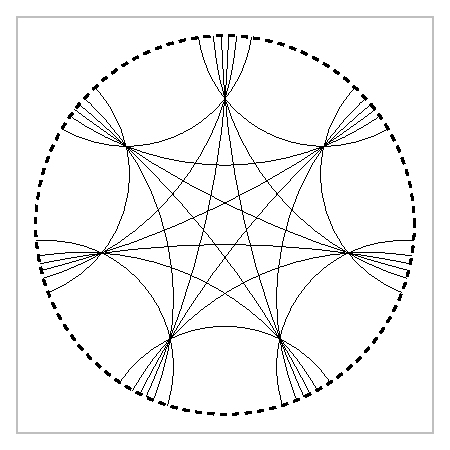
\includegraphics[scale=1.8,trim=4 4 4 4,clip]{src/geo/gfx/cover/cover.eps}
\end{center}

\newpage
\tableofcontents

\setcounter{page}{0}

\begin{center}
\begin{minipage}{0.8\textwidth}
\begin{center}
\vspace{40pt}

This work is licensed under a Creative Commons Attribution NonCommercial ShareAlike 4.0 International License.

\vspace{12pt}

\includegraphics[scale=0.8]{src/geo/gfx/by-nc-sa.eps}
\end{center}
\end{minipage}
\end{center}
\newpage


\mainmatter

\chapter{Incidence}
\newpage

  \section{Models and Theories}
    One of the goals of this class is to explore the classical theory of geometry as laid out in the famous \emph{Elements of Geometry} by the Greek mathematician Euclid.
Before we begin, though, a few words about the distinction between a \emph{theory} and a \emph{model} are in order.

\begin{itemize}
\item A \textbf{theory} consists of one or more \emph{undefined terms}, which are used in one or more \emph{axioms} or \emph{definitions}, which are then the basis for a list of logical deductions called \emph{theorems}.
This may be how you think about geometry as you learned it in high school.

\item A \textbf{model} is a concrete realization of a theory: a way to associate the undefined terms to ``real'' objects such that the axioms are satisfied.
Models are where we perform calculations and draw pictures.
\end{itemize}

The correspondence between theories and models is not one-to-one (in either direction).
There are theories which have many models, other theories with exactly one model, and yet other theories which have no models at all.
Conversely, a given concrete object is likely a model of many different theories, though not all of them will be interesting.

The difference between theory and model turns out to have significant practical applications.
In the real world we compute with concrete objects -- things like numbers and sets.
This is useful, but concrete objects have a tendency to get very messy very quickly.
However if some aspects of a concrete object are a model for some theory, we can ``throw away'' unimportant details and compute more easily at an abstract level.
For instance many important theorems about matrices are difficult and tedious to prove if we think of matrices as arrays of numbers but become simple if we think of matrices as linear transformations.

An example of a theory which you may have seen before is Euclid's postulates for geometry.
These are a small number of statements which Euclid took to be obviously true (\emph{axioms} in modern lingo) such as ``two points determine a line'' and so on.
Euclid developed this theory of geometry in a book, called \emph{The Elements}, which went on to become a standard mathematical textbook for many centuries.

The development and proliferation of Euclid's geometry predates the recognition of the need to carefully distinguish between a theory and its models, and early work did not make this distinction.
Euclid seems to have written under the assumption that the universe comes equipped with exactly one geometry -- that his theory has only one model.
Unfortunately for us, this early confusion led to some problems.
First, it turns out that there are many models of geometry, some of which are very strange.
We will explore several models of geometry in this text.

The second problem we inherit from Euclid is more serious.
Because he conflated his \emph{theory} of geometry with only one particular \emph{model}, and this confusion was not cleared up until much later, and because his book was so influential, Euclid left us with a language problem.
The basic terms of geometry -- point, line, circle, segment, angle -- have multiple meanings.
There is the meaning inside Euclid's \emph{model} of geometry, which corresponds mostly to the bits of geometry we use in college algebra and calculus.
But these words have another, more abstract meaning inside Euclid's \emph{theory} of geometry, and when these terms are used inside other models we can easily get confused.
We will look at models of geometry where lines are circles, where points are lines, and where circles are ellipses.

\subsection*{Theories as Languages}

We can think of a theory as a kind of abstract \emph{language}.
The undefined terms are the words -- nouns, verbs, and so on -- while the axioms are the grammar, specifying how the words can be put together into meaningful phrases.

Unlike a natual language, logical theories are very well suited to implementation in software.
So, for example, a valid ``sentence'' expressed in a geometric theory-language can be turned into a drawing by machine.
This idea is not new, but it is very powerful.



%---------%
\Exercises%
%---------%

\begin{exercise}\label{exerc:rr-between-sign}
Let \(\alpha, \beta \in \RR\) and \(t \in (0,1)\).
\begin{proplist}
\item If \(\alpha > 0\) and \(\beta > 0\), then \(\alpha + t(\beta - \alpha) > 0\).
\item If \(\alpha > 0\) and \(\beta > 0\), then \(\alpha + t(\beta - \alpha) < 0\).
\end{proplist}
\end{exercise}


\begin{exercise}\label{exerc:rr-between-square}
Let \(\alpha\), \(\beta\), and \(\gamma\) be in \(\RR\) such that \(\alpha < \beta < \gamma\).
Show that either \(\beta^2 < \alpha^2\) or \(\beta^2 < \gamma^2\).
\end{exercise}

    \newpage

  \section{Incidence Geometry}
    Traditional plane geometry involves many different concepts, including \emph{lines}, \emph{angles}, \emph{congruent}, and many others.
In order to manage the complexity this entails, we will build up our geometries one piece at a time starting here with the idea of \emph{collinearity}.

\begin{dfn}[Incidence Geometry] \label{dfn:incidence-geometry}
Let \(P\) be a set, whose elements we call \emph{points}.
A ternary relation \(\COLLINEAR{\ast}{\ast}{\ast}\) on \(P\) is called a \emph{collinearity relation}\index{collinearity} if the following properties are satisfied.
\begin{proplist}
\item[IG1.] If \(a\), \(b\), and \(c\) are points such that \(\COLLINEAR{a}{b}{c}\), then \(\COLLINEAR{b}{a}{c}\) and \(\COLLINEAR{a}{c}{b}\).
\item[IG2.] If \(a\) and \(b\) are points such that \(a \neq b\), then \(\COLLINEAR{a}{b}{b}\).
\item[IG3.] \(\COLLINEAR{a}{a}{a}\) does not hold for any point \(a\).
\item[IG4.] There exist distinct points \(a\), \(b\), and \(c\) such that \(\COLLINEAR{a}{b}{c}\) does not hold.
\item[IG5.] \textbf{Exchange Property:} If \(a\), \(b\), \(u\), and \(v\) are points such that \(a \neq b\), \(u \neq v\), \(\COLLINEAR{a}{b}{u}\), and \(\COLLINEAR{a}{b}{v}\), then \(\COLLINEAR{a}{u}{v}\).
\end{proplist}
If such a relation exists we say that \((P, \COLLINEAR{\ast}{\ast}{\ast})\) is an \emph{incidence geometry}\index{incidence geometry}.
In this case, when \(\COLLINEAR{a}{b}{c}\) we say that \(a\), \(b\), and \(c\) are \emph{collinear}.
\end{dfn}

It is important to remember that the word ``collinear'' here is an undefined term, and we have to try very hard not to think of ordinary lines and points when using it.
(This is part of the theory-model confusion we inherit from history.)
The meaning of the word ``collinear'' is determined precisely by how it is used in the incidence geometry axioms, and only becomes concrete when we specify a particular model.
In particular, it does not make sense to draw pictures of the points in an arbitrary incidence geometry!

Although ``collinear'' is an abstract, undefined term, we'd like for it to behave much like our intuition expects.
We want this undefined term to \emph{formalize} our intuition about collinearity.
To that end, note that collinearity satisfies some additional basic properties.

\begin{prop}
Let \(P\) be an incidence geometry.
Then we have the following for all points \(a\), \(b\), and \(c\).
\begin{proplist}
\item If \(\COLLINEAR{a}{b}{c}\), then we also have \(\COLLINEAR{b}{c}{a}\), \(\COLLINEAR{c}{a}{b}\), and \(\COLLINEAR{c}{b}{a}\).
\item If \(a \neq b\), then \(\COLLINEAR{a}{b}{a}\) and \(\COLLINEAR{b}{a}{a}\).
\end{proplist}
\end{prop}

It may seem strange to define ``collinear'' before we define ``line''; typically we think of points being collinear precisely when there is a unique line containing all of them.
But we can just as easily define lines in terms of collinearity as follows.

\begin{dfn}[Line] \label{dfn:line}
Let \(P\) be an incidence geometry with distinct points \(a\) and \(b\).
We define the \emph{line}\index{line} through \(a\) and \(b\) to be the set \[ \LINE{a}{b} = \{ c \in P \mid \COLLINEAR{a}{b}{c} \}. \]
If \(c \in \LINE{a}{b}\), we say that \(c\) \emph{lies on} \(\LINE{a}{b}\).
\end{dfn}

That is, the line through \(a\) and \(b\) is precisely the set of points which are collinear with \(a\) and \(b\).
Remember: it is vital that we not think about drawings of points and lines here.
In an arbitrary incidence geometry, ``point'' and ``line'' are just \emph{words} which we assume have a particular relationship with one another.
Thinking at this level of abstraction may seem unnecessarily difficult at first, but -- and it is difficult to overstate this -- the abstract way of thinking brings enormous power.
Here are some basic properties of lines which can be derived from the properties of collinearity alone.

\begin{prop}
Let \(P\) be an incidence geometry.
Then the following hold for all distinct points \(a\) and \(b\) in \(P\).
\begin{proplist}
\item \(a \in \LINE{a}{b}\) and \(b \in \LINE{a}{b}\).
\item \(\LINE{a}{b} = \LINE{b}{a}\).
\item If \(c \in \LINE{a}{b}\) and \(c \neq a\), then \(\LINE{a}{c} = \LINE{a}{b}\).
\item If \(u,v \in \LINE{a}{b}\) are distinct points, then \(a,b \in \LINE{u}{v}\).
\end{proplist}
\end{prop}

Though we will eventually have several examples of incidence geometry, it is crucial when proving theorems that we not rely on any specific model.
This is the power of abstraction: any theorem which depends only on properties common to \emph{all} incidence geometries immediately holds in \emph{any} incidence geometry.
For example, consider the following theorem.

\begin{prop}[Line Intersection]
Let \(P\) be an incidence geometry with lines \(\ell_1\) and \(\ell_2\).
Then exactly one of the following holds.
\begin{proplist}
\item \(\ell_1 = \ell_2\), and we say \(\ell_1\) and \(\ell_2\) are \emph{coincident}\index{coincident lines},
\item \(\ell_1 \cap \ell_2 = \varnothing\), and we say \(\ell_1\) and \(\ell_2\) are \emph{disjoint}\index{disjoint lines}, or
\item \(\ell_1 \cap \ell_2 = \{p\}\) for some point \(p\), and we say \(\ell_1\) and \(\ell_2\) are \emph{incident}\index{incident lines}.
\end{proplist}
In the first two cases (coincident or disjoint) we say that \(\ell_1\) and \(\ell_2\) are \emph{parallel}\index{parallel lines}.
\end{prop}

\begin{proof}
Suppose \(\ell_1 \cap \ell_2\) contains at least two points, say \(x\) and \(y\).
Then in fact \(\ell_1 = \LINE{x}{y} = \ell_2\).
So if \(\ell_1 \neq \ell_2\) then \(\ell_1 \cap \ell_2\) contains either exactly one or zero points.
\end{proof}

This theorem holds in any model of incidence geometry.
One problem: we don't have any models of incidence geometry yet!
We'll fix this in the next section.



%---------%
\Exercises%
%---------%

\begin{exercise}\label{exerc:rr2-collinear-comb}
Let \(A = (a_x, a_y)\), \(B = (b_x, b_y)\), and \(C = (c_x, c_y)\) be in \(\RR^2\) such that \(A \neq B\).
Show that \[ \DET \begin{bmatrix} a_x & a_y & 1 \\ b_x & b_y & 1 \\ c_x & c_y & 1 \end{bmatrix} = 0 \] if and only if \(C = A + t(B - A)\) for some unique \(t \in \RR\).
(Hint: Consider the expression \( (c_x - a_x)/(b_x - a_x) = (c_y - a_y)/(b_y - a_y) \).)
\end{exercise}

    \newpage

  \section{Parallel Lines}
    Recall that two lines in an incidence geometry are called \emph{parallel} if they do not meet at a single point.
The following question about parallel lines turns out to be interesting.
\begin{titlebox}{Question}
\begin{center}
Suppose we have a line \(\ell\) and a point \(p\) in an incidence geometry.
How many lines exist which pass through \(p\) and are parallel to \(\ell\)?
\end{center}
\end{titlebox}
Our intuition says that the answer to this question is clearly 1, and Euclid agreed.
It turns out that the parallel lines in our models so far behave in some very different ways.


\subsection{Parallels in \(\RR^2\)}

In \eref{exerc:parallels-in-rr2} we found a nice way to characterize whether the lines determined by four cartesian points are parallel: if \(A = (a_x, a_y)\), \(B = (b_x, b_y)\), \(C = (c_x, c_y)\), and \(D = (d_x, d_y)\) are points in \(\RR^2\) with \(A \neq B\) and \(C \neq D\), then \(\LINE{A}{B} \parallel \LINE{C}{D}\) if and only if \[ \DET \begin{bmatrix} b_x - a_x & d_x - c_x \\ b_y - a_y & d_y - c_y \end{bmatrix} = 0. \]
With this, we can show the following.

\begin{prop}
If \(\ell = \LINE{A}{B}\) is a line and \(C \notin \ell\) a point in \(\RR^2\), then there is exactly one line passing through \(C\) which is parallel to \(\ell\).
\end{prop}

\begin{proof}
To see existence, let \(D = C + B - A\).
Now \(D \neq C\) since \(B \neq A\).
Moreover, \(\LINE{C}{D}\) and \(\LINE{A}{B}\) are parallel since \[ \DET \begin{bmatrix} b_x - a_x & c_x + b_x - a_x - c_x \\ b_y - a_y & c_y + b_y - a_y - c_y \end{bmatrix} = \DET \begin{bmatrix} b_x - a_x & b_x - a_x \\ b_y - a_y & b_y - a_y \end{bmatrix} = 0. \]
To see uniqueness, suppose \(X = (x, y)\) is a point (different from \(C\)) such that \(\LINE{C}{X}\) is parallel to \(\LINE{A}{B}\).
Then \[ 0 = \DET \begin{bmatrix} x - c_x & b_x - a_x \\ y - c_y & b_y - c_y \end{bmatrix} = \DET \begin{bmatrix} x - c_x & c_x + b_x - a_x - c_x \\ y - c_y & c_y + b_y - a_y - c_y \end{bmatrix}. \]
So \(X\), \(C\), and \(D\) are collinear, and thus \(\LINE{C}{X} = \LINE{C}{D}\).
\end{proof}

This proof remains valid in the rational plane.


\subsection{Parallels in \(\mathbb{D}\)}

Suppose \(\ell\) is a line and \(x\) a point in the unit disc.
There are \emph{infinitely many} lines passing through \(x\) which are parallel to \(\ell\).
To see why, remember that \(\ell\) is contained in a line \(\ell_{A,B}\) in the Cartesian Plane.
Choose any point \(y\) on this Cartesian line which is not in the unit disk, and let \(\ell_{x,y}\) be the Cartesian line generated by \(x\) and \(y\).
Now \(\ell' = \ell_{x,y} \cap \mathbb{D}\) is parallel to \(\ell\).



\subsection{Parallels in \(\mathbb{A}\)}

It is not too difficult to see that there are \emph{no} pairs of parallel lines in the antipodal sphere; any two different great circles have to intersect.




\subsection{Parallels in the Fano plane}

In the Fano Plane, no two lines are parallel.
In particular, if \(\ell\) is a line and \(x \notin \ell\) a point, there are \emph{no} lines passing through \(x\) which are parallel to \(\ell\).



Considering these examples, there seem to be (at least) three qualitatively different possibilities for the answer to our Question about parallel lines.
This observation is what motivates the following definition.

\begin{dfn}[The Parallel Postulates]
We say that an incidence geometry \(P\) is
\begin{description}
\item[Elliptic] if there are \emph{no} lines passing through \(x\) and parallel to \(\ell\), for all lines \(\ell\) and points \(x \notin \ell\).
\item[Euclidean] if there is \emph{exactly one} line passing through \(x\) and parallel to \(\ell\), for all lines \(\ell\) and points \(x \notin \ell\).
\item[Hyperbolic] if there are \emph{infinitely many} lines passing through \(x\) and parallel to \(\ell\), for all lines \(\ell\) and points \(x \notin \ell\).
\end{description}
\end{dfn}

With this definition, \(\RR^2\) and \(\QQ^2\) are Euclidean, \(\mathcal{F}\) and \(\mathbb{A}\) are Elliptic, and \(\mathbb{D}\) and \(\mathbb{H}\) are Hyperbolic.
It is important to note that a given incidence geometry need not satisfy \textbf{any} of these properties!
We will see a strange example of this in the exercises.



\subsection*{Transitivity of Parallelism}

The kinds of ``geometries'' that arise from our three different Parallel Postulates will be different -- perhaps drastically so -- as illustrated by the following result.

\begin{prop}
Suppose \(P\) is a Euclidean incidence geometry, with lines \(\ell_1\), \(\ell_2\), and \(\ell_3\).
If \(\ell_1 \parallel \ell_2\) and \(\ell_2 \parallel \ell_3\), then \(\ell_1 \parallel \ell_3\).
That is, the relation ``is parallel to'' is transitive.
\end{prop}

\begin{proof}
If \(\ell_1 \cap \ell_2 = \varnothing\), then \(\ell_1 \parallel \ell_3\) by definition.
Suppose instead that \(\ell_1\) and \(\ell_3\) have \emph{at least one} point in common, say \(p\).
Since \(\ell_1\) is parallel to \(\ell_2\), note that \(p \notin \ell_2\).
Since \(\mathcal{P}\) is Euclidean, there is exactly one line passing through \(p\) which is parallel to \(\ell_2\); call this line \(\ell\).
But now \(\ell_1\) is a line parallel to \(\ell_2\) which passes through \(p\), so that \(\ell_1 = \ell\).
Likewise, \(\ell_3 = \ell\).
Hence \(\ell_1 = \ell_3\), and so \(\ell_1 \parallel \ell_3\) as claimed.
\end{proof}

Note that in a Hyperbolic incidence geometry, this need not be the case.
If we have two lines \(\ell_1\) and \(\ell_3\) which pass through a point \(p\) and are parallel to a given line \(\ell_2\), then \(\ell_1\) and \(\ell_3\) are \emph{not} parallel.
And in an Elliptic incidence geometry the transitivity of parallelism is irrelevant: there are no pairs of distinct parallel lines to begin with.



%---------%
\Exercises%
%---------%

Note that although all of our example incidence geometries happen to be either elliptic, euclidean, or hyperbolic, any given incidence geometry need not be in any of these classes.
The next two exercises construct an example.

\begin{dfn}[The Two-Pointed Line]
Let \(P = \RR \cup \{A,B\}\), where we think of \(A\) and \(B\) simply as symbols not belonging to \(\RR\).
We define a ternary relation on \(P\) as follows.
Given points \(x,y,z \in P\), not all equal, we say that \(\COLLINEAR{x}{y}{z}\) if one of the following holds.
\begin{proplist}
\item \(\{x,y,z\} \subseteq \RR\).
\item \(\{x,y,z\} = \{A,\zeta\}\) for some \(\zeta \in \RR\).
\item \(\{x,y,z\} = \{B,\zeta\}\) for some \(\zeta \in \RR\).
\item \(\{x,y,z\} = \{A,B\}\).
\end{proplist}
We refer to this structure as the Two-Pointed Line.
\end{dfn}

\begin{exercise}
Show that the Two-Pointed Line is an incidence geometry.
\end{exercise}

\begin{exercise}
Show that the Two-Pointed Line is an incidence geometry which is neither elliptic, nor euclidean, nor hyperbolic as follows.
\begin{proplist}
\item Find a line \(\ell\) and a point \(x\) in the Two-Pointed Line such that there is exactly one line passing through \(x\) and parallel to \(\ell\).
\item Find a line \(\ell\) and a point \(x\) in the Two-Pointed Line such that there are infinitely many lines passing through \(x\) and parallel to \(\ell\).
\end{proplist}
\end{exercise}

    \newpage

  \section{Collineations}
    Collinearity relations represent a kind of \emph{abstract structure}.
Typically in mathematics, whenever we have a kind of structure, the mappings which \emph{preserve} that structure are interesting.
In the case of an incidence geometry such mappings are called \emph{collineations}.

\begin{dfn}[Collineation]
Suppose we have incidence geometries \(P\) and \(Q\).
A bijective mapping \(\varphi : P \rightarrow Q\) is called a \emph{collineation}\index{collineation} if, for all points \(x,y,z \in P\), whenever \(\COLLINEAR{x}{y}{z}\) in \(P\), we also have \(\COLLINEAR{\varphi(x)}{\varphi(y)}{\varphi(z)}\) in \(Q\).
\end{dfn}

\begin{prop}
We have the following.
\begin{proplist}
\item If \(P\) is an incidence geometry, then the identity map \(1 : P \rightarrow P\) is a collineation.
\item If \(\varphi : P \rightarrow Q\) and \(\psi : Q \rightarrow R\) are collineations, then \(\psi \circ \varphi\) is a collineation.
\item If \(\varphi : P \rightarrow Q\) is a collineation, then \(\varphi^{-1} : Q \rightarrow P\) is a collineation.
\end{proplist}
\end{prop}



%---------%
\Exercises%
%---------%

\begin{exercise}
Let \(\varphi : \RR^2 \rightarrow \RR^2\) be given by \[ \varphi(X) = MX + B, \]
where \(M\) is an invertible \(2 \times 2\) matrix over \(\RR\) and \(B \in \RR^2\).
Show that \(\varphi\) is a collineation.
\end{exercise}



\chapter{Order}
\newpage

  \section{Betweenness}
    In an incidence geometry we have the ability to detect whether three given points are collinear.
However an arbitrary incidence geometry has no notion of ``order'' for the points on a given line, as we might intuitively expect.
For instance, the points \((0,0)\), \((1,1)\), and \((2,2)\) are collinear in \(\RR^2\) and we think of \((1,1)\) as being ``between'' the other two.
But in the Fano plane, does it make sense to order the points on a line?
Presently we introduce another piece of technology to an incidence geometry which will allow us to formalize the concept of ``betweenness''.

\begin{dfn}[Betweenness]
Let \(P\) be an incidence geometry.
We say that a ternary relation \(\BETWEEN{\ast}{\ast}{\ast}\) on \(P\) is a \emph{betweenness relation}\index{betweenness} if the following properties hold.
\begin{proplist}
\item[B1.] If \(\BETWEEN{x}{y}{z}\), then \(x\), \(y\), and \(z\) are distinct and \(\COLLINEAR{x}{y}{z}\).
\item[B2.] If \(\BETWEEN{x}{z}{y}\), then \(\BETWEEN{y}{z}{x}\).
\item[B3.] If \(x\), \(y\), and \(z\) are distinct points such that \(\COLLINEAR{x}{y}{z}\), then at least one of \(\BETWEEN{x}{y}{z}\), \(\BETWEEN{y}{z}{x}\), and \(\BETWEEN{z}{x}{y}\) is true.
\item[B4.] If \(\BETWEEN{x}{y}{z}\) and \(\BETWEEN{x}{z}{w}\), then \(\BETWEEN{x}{y}{w}\) and \(\BETWEEN{y}{z}{w}\).
\item[B5.] If \(\BETWEEN{x}{y}{z}\) and \(\BETWEEN{y}{z}{w}\), then \(\BETWEEN{x}{y}{w}\) and \(\BETWEEN{x}{z}{w}\).
\item[B6.] \textbf{Interpolation Property:} If \(x\) and \(y\) are distinct points, then there exist points \(z_1\), \(z_2\), and \(z_3\) such that \(\BETWEEN{z_1}{x}{y}\), \(\BETWEEN{x}{z_2}{y}\), and \(\BETWEEN{x}{y}{z_3}\).
\end{proplist}
\end{dfn}

If \(\BETWEEN{x}{y}{z}\), we say that \(z\) is \emph{between} \(x\) and \(y\).
B1 says that ``betweenness'' is a refinement of ``collinearity''.
B2 says that betweenness is symmetric (if we fix the middle point).
B3 says that distinct collinear points must be in order somehow, outlawing the bizarre situation where points are collinear but not in order.
B4 and B5 are a little more interesting; they are a kind of coherence condition for betweenness.
Consider a situation like \autoref{fig:betweenness-coherence}.
Axiom B4 says that if \(y\) is between \(x\) and \(z\) and \(z\) is between \(x\) and \(w\), then \(y\) is between \(x\) and \(w\) and \(z\) is between \(y\) and \(w\).
That seems reasonable enough, and B5 says something similar.

\begin{figure}
\begin{center}
\begin{tikzpicture}
  \coordinate [label=below:\(x\)] (X) at (0,0);
  \coordinate [label=below:\(y\)] (Y) at (1,0.5);
  \coordinate [label=below:\(z\)] (Z) at (2,1);
  \coordinate [label=below:\(w\)] (W) at (3,1.5);

  \draw [fill] (X) circle [radius=1pt];
  \draw [fill] (Y) circle [radius=1pt];
  \draw [fill] (Z) circle [radius=1pt];
  \draw [fill] (W) circle [radius=1pt];

  \draw [<->] (-1,-0.5) -- (4,2);
\end{tikzpicture}
\caption{\label{fig:betweenness-coherence}The coherence conditions B4 and B5.}
\end{center}
\end{figure}

As shorthand, if \(x\), \(y\), \(z\), and \(w\) are distinct points, we will say \([xyzw]\) precisely when \(\BETWEEN{x}{y}{z}\), \(\BETWEEN{x}{y}{w}\), \(\BETWEEN{x}{z}{w}\), and \(\BETWEEN{y}{z}{w}\).
More generally, if \(x_1, \ldots, x_n\) are distinct points, then \([x_1x_2 \ldots x_n]\) means that \(\BETWEEN{x_i}{x_j}{x_k}\) for all triples \((i,j,k)\) with \(1 \leq i < j < k \leq n\).
The next definition will probably look familiar.

\begin{dfn}[Segment, Ray]
Let \(x\) and \(y\) be points in an incidence geometry \(P\) with a betweenness relation.
\begin{proplist}
\item The set \[ \SEGMENT{x}{y} = \{ z \in P \mid z = x\ \mathrm{or}\ z = y\ \mathrm{or}\ \BETWEEN{x}{z}{y} \} \] is called the \emph{segment}\index{segment} with \emph{endpoints} \(x\) and \(y\).
If \(x = y\) we say that the segment \(\SEGMENT{x}{y}\) is \emph{degenerate}.
If \(z \in \SEGMENT{x}{y}\) and \(z \neq x\) and \(z \neq y\), we say that \(z\) is \emph{interior to}\index{interior!of a segment} \(\SEGMENT{x}{y}\).
\item The set \[ \RAY{x}{y} = \{ z \in P \mid z = x\ \mathrm{or}\ z = y\ \mathrm{or}\ \BETWEEN{x}{z}{y}\ \mathrm{or}\ \BETWEEN{x}{y}{z} \} \] is called the \emph{ray}\index{ray} with \emph{vertex} \(x\) \emph{toward} \(y\).
If \(x = y\) we say that the ray \(\RAY{x}{y}\) is \emph{degenerate}.
If \(z \in \RAY{x}{y}\) and \(z \neq x\), we say that \(z\) is \emph{interior to}\index{interior!of a ray} \(\RAY{x}{y}\).
\end{proplist}
\end{dfn}

The following properties of segments and rays essentially fall out of the definition.

\begin{prop}
If \(P\) is an incidence geometry and \(\BETWEEN{\cdot}{\cdot}{\cdot}\) a betweenness relation on \(P\), then the following hold.
\begin{enumerate}
\item \(\SEGMENT{x}{y} = \SEGMENT{y}{x}\) for all distinct points \(x\) and \(y\).
\item \(\SEGMENT{x}{y} \subseteq \RAY{x}{y} \subseteq \LINE{x}{y}\) for all distinct points \(x\) and \(y\).
\item If \(\ell\) is a line and \(x\) and \(y\) distinct points, then \(\SEGMENT{x}{y} \cap \ell\) is either \(\SEGMENT{x}{y}\), \(\varnothing\), or \(\{p\}\) for some point \(p\).
\item \(\RAY{x}{y} \cap \RAY{y}{x} = \SEGMENT{x}{y}\) for all distinct points \(x\) and \(y\).
\end{enumerate}
\end{prop}



\begin{prop}[Line Decomposition]\label{prop:line-decomp}
Suppose \(P\) is an incidence geometry with a betweenness relation, and let \(x,y \in P\) be distinct points.
Then \[ \LINE{x}{y} = \{ z \in P \mid z = x\ \mathrm{or}\ z = y\ \mathrm{or}\ \BETWEEN{z}{x}{y}\ \mathrm{or}\ \BETWEEN{x}{z}{y}\ \mathrm{or}\ \BETWEEN{x}{y}{z} \}. \]
\end{prop}

Proposition \ref{prop:line-decomp} is a useful technical result: if we know that a given point \(z\) lies on a line \(\ell_{x,y}\), then there are five possibilities.
The next result is useful for the same reason.

\begin{prop}
Let \(P\) be an incidence geometry with a betweenness relation and suppose \(x\), \(y\), \(z\), and \(w\) are points.
If \(\BETWEEN{x}{z}{y}\) and \(\BETWEEN{x}{w}{y}\), then either \(\BETWEEN{x}{z}{w}\) or \(\BETWEEN{x}{w}{z}\) or \(z = w\).
\end{prop}

We can now define \emph{convexity} in terms of betweenness as follows.

\begin{dfn}[Convexity]
Let \(P\) be an incidence geometry with a betweenness relation.
A non empty set \(S\) of points in \(P\) is called \emph{convex}\index{convex} if it is closed under betweenness in the following sense: if \(x,y \in S\) and \(\BETWEEN{x}{z}{y}\), then \(z \in S\).
\end{dfn}



%---------%
\Exercises%
%---------%

\begin{exercise}
Suppose \(P\) is an incidence geometry with a betweenness relation.
If \(x\), \(y\), and \(z\) are distinct points such that \(\BETWEEN{x}{y}{z}\), then the following hold.
\begin{proplist}
\item \(\SEGMENT{x}{y} \cup \SEGMENT{y}{z} = \SEGMENT{x}{z}\).
\item \(\SEGMENT{x}{y} \cap \SEGMENT{y}{z} = \{y\}\).
\item \(\RAY{y}{x} \cap \RAY{y}{z} = \{y\}\).
\item \(\RAY{x}{y} = \RAY{x}{z}\).
\item \(\RAY{x}{y} \cap \RAY{y}{x} = \SEGMENT{x}{y}\).
\item \(\RAY{y}{x} \cup \RAY{y}{z} = \LINE{x}{z}\).
\end{proplist}
\end{exercise}

\begin{exercise}
Let \(P\) be an incidence geometry with a betweenness relation, and let \(S \subseteq P\).
Show that \(S\) is convex if and only if \(\SEGMENT{x}{y} \subseteq S\) for all distinct points \(x,y \in S\).
\end{exercise}

\begin{exercise}
Let \(P\) be an incidence geometry with a betweenness relation and \(x,y \in P\) distinct points.
Show that the following sets are convex.
\begin{proplist}
\item \(\LINE{x}{y}\)
\item \(\SEGMENT{x}{y}\)
\item \(\RAY{x}{y}\)
\end{proplist}
\end{exercise}

\begin{exercise}
Let \(P\) be an incidence geometry with a betweenness relation.
Show that every line in \(P\) contains infinitely many points.
\end{exercise}

    \newpage

  \section{Ordered Geometry}
    The existence of a betweenness relation on an incidence geometry says something very strong.
Combined with an additional property -- the Line Separation property -- such geometries are called \emph{ordered}.

\begin{dfn}[Ordered Geometry]
Let \(P\) be an incidence geometry with a betweenness relation \(\BETWEEN{\ast}{\ast}{\ast}\).
We say that \(P\) is an \emph{ordered geometry} if it satisfies the following additional \emph{Line Separation Property}.
\begin{itemize}
\item[LS.] For every line \(\ell\) there are two sets, \(\HALFPLANEA{\ell}\) and \(\HALFPLANEB{\ell}\), which satisfy the following properties.
\begin{proplist}
\item \(\HALFPLANEA{\ell}\) and \(\HALFPLANEB{\ell}\) are not empty.
\item \(\ell\), \(\HALFPLANEA{\ell}\), and \(\HALFPLANEB{\ell}\) partition \(P\).
\item \(\HALFPLANEA{\ell}\) and \(\HALFPLANEB{\ell}\) are convex.
\item If \(x \in \HALFPLANEA{\ell}\) and \(y \in \HALFPLANEB{\ell}\), then \(\SEGMENT{x}{y} \cap \ell = \{p\}\) for some point \(p\).
\end{proplist}
The sets \(\HALFPLANEA{\ell}\) and \(\HALFPLANEB{\ell}\) are called \emph{halfplanes}\index{halfplane}.
\end{itemize}
\end{dfn}

The Line Separation property essentially states that every line divides the plane into two ``separate'' pieces -- we might call these pieces the \emph{sides} of the line.
Given a line \(\ell\) and points \(x,y \notin \ell\), we say that \(x\) and \(y\) are on the \emph{same side} of \(\ell\) if they are both in the same halfplane bounded by \(\ell\), and otherwise they are on \emph{opposite sides}.
See \autoref{fig:line-sep} for a picture.
(But remember that a given ordered geometry might look very different!)

\begin{figure}[h]
\begin{center}
\begin{tikzpicture}
  \draw [<->] (0,0) -- (2,4);
  \coordinate [label=below right:\(\ell\)] (x) at (1,2);
  \node at (-1,2) {\(\HALFPLANEA{\ell}\)};
  \node at (2.5,2) {\(\HALFPLANEB{\ell}\)};
\end{tikzpicture}
\caption{\label{fig:line-sep}The halfplanes bounded by a line.}
\end{center}
\end{figure}

\begin{dfn}[Triangle]
Let \(P\) be an incidence geometry, and let \(x\), \(y\), and \(z\) be points.
Then the set \[ \TRIANGLE{x}{y}{z} = \SEGMENT{x}{y} \cup \SEGMENT{y}{z} \cup \SEGMENT{z}{x} \] is called the \emph{triangle} with \emph{vertices} \(x\), \(y\), and \(z\).
The segments \(\SEGMENT{x}{y}\), \(\SEGMENT{y}{z}\), and \(\SEGMENT{z}{x}\) are called the \emph{sides}\index{sides (of a triangle)} of the triangle, and the lines \(\LINE{x}{y}\), \(\LINE{y}{z}\), and \(\LINE{z}{x}\) are called the \emph{extended sides}\index{extended sides (of a triangle)}.
If \(x\), \(y\), and \(z\) are not all distinct, we say that the triangle \(\TRIANGLE{x}{y}{z}\) is \emph{degenerate}\index{degenerate!triangle}.
\end{dfn}

The next result seems intuitive, but must be proven; it states that if a line ``enters'' a triangle through one side and does not contain any of the triangle's vertices, then it must ``exit'' the triangle through one of the other sides.
This is called \emph{Pasch's Axiom} for historical reasons.

\begin{prop}[Pasch's Axiom]
Let \(x\), \(y\), and \(z\) be distinct noncollinear points in an ordered geometry, and let \(\ell\) be a line such that \(x,y,z \notin \ell\).
Finally, suppose there is a point \(w \in \ell\) such that \(\BETWEEN{x}{w}{y}\); that is, \(\ell\) cuts the side \(\SEGMENT{x}{y}\).
Then precisely one of the following two things happens:
\begin{proplist}
\item \(\ell\) cuts \(\SEGMENT{y}{z}\) and does not cut \(\SEGMENT{z}{x}\), or
\item \(\ell\) cuts \(\SEGMENT{z}{x}\) and does not cut \(\SEGMENT{y}{z}\).
\end{proplist}
\end{prop}

\begin{proof}
Since \(P\) is an ordered geometry, it satisfies the Plane Separation property.
In particular, the points not on \(\ell\) are partitioned into two convex, nonempty half-planes, \(\HALFPLANEA{\ell}\) and \(\HALFPLANEB{\ell}\).
Since \(x\) and \(y\) are not on \(\ell\), without loss of generality we have \(x \in \HALFPLANEA{\ell}\) and \(y \in \HALFPLANEB{\ell}\).
Since \(z \notin \ell\), there are two possibilities: either \(z \in \HALFPLANEA{\ell}\) or \(z \in \HALFPLANEB{\ell}\).
In the first case, we see that \(\ell\) cuts \(\SEGMENT{y}{z}\) and does not cut \(\SEGMENT{z}{x}\), and in the second case, \(\ell\) cuts \(\SEGMENT{z}{x}\) but not \(\SEGMENT{y}{z}\).
\end{proof}

In other words, Pasch's Axiom states that if a line enters a triangle then it must also exit; see Figure \ref{fig:pasch}.

\begin{figure}[h]
\begin{center}
\begin{tikzpicture}[scale=1.1]
  \coordinate [label=below:\(x\)] (X) at (0,0);
  \coordinate [label=above left:\(y\)] (Y) at (-1,2);
  \coordinate [label=right:\(z\)] (Z) at (4,1);
  \coordinate (H) at (0,1);
  \coordinate (K) at (-2,2);
  \draw (X) -- (Y) -- (Z) -- cycle;
  \draw [->] (H) -- (K);
  \coordinate [label=below left:\(w\)] (W) at (intersection of X--Y and H--K);
  \draw [->,dashed] (H) -- (1,0.5);
  \draw [fill] (X) circle [radius=0.7pt];
  \draw [fill] (Y) circle [radius=0.7pt];
  \draw [fill] (Z) circle [radius=0.7pt];
  \draw [fill] (W) circle [radius=0.7pt];
\end{tikzpicture}
\caption{\label{fig:pasch}The setup of Pasch's Axiom}
\end{center}
\end{figure}

\begin{lem}\label{lem:betweenness-separation}
Let \(\ell\) be a line and \(C \in \ell\) a point in an ordered geometry.
Suppose \(A\) and \(B\) are points not on \(\ell\) such that \(\BETWEEN{A}{B}{C}\).
Then \(A\) and \(B\) are on the same side of \(\ell\).
\end{lem}

\begin{proof}
Suppose otherwise that \(A\) and \(B\) are on opposite sides of \(\ell\).
By the Line Separation property, and because \(A\) and \(B\) are not on \(\ell\), the segment \(\SEGMENT{A}{B}\) cuts \(\ell\) at a unique point \(D\).
That is, \(D \in \ell\) and \(\BETWEEN{A}{D}{B}\).
In particular, \(D\) and \(C\) must be distinct since we have \(\BETWEEN{D}{B}{C}\).
But note that \(C, D \in \ell\), so \(\LINE{C}{D} = \ell\), and also \(C, D \in \LINE{A}{B}\), so that \(\LINE{C}{D} = \LINE{A}{B}\).
But then \(\LINE{A}{B} = \ell\), a contradiction.
Thus \(A\) and \(B\) must be on the same side of \(\ell\).
\end{proof}



%---------%
\Exercises%
%---------%

\begin{exercise}
Let \(a\), \(b\), and \(c\) be distinct noncollinear points.
Suppose we have points \(d\) and \(e\) such that \(\BETWEEN{a}{b}{d}\) and \(\BETWEEN{a}{e}{c}\).
Then there exists a point \(f\) such that \(\BETWEEN{e}{f}{d}\) and \(\BETWEEN{b}{f}{c}\).
\end{exercise}

\begin{exercise}
Let \(a\), \(b\), and \(c\) be distinct noncollinear points.
Suppose we have points \(d\) and \(e\) such that \(\BETWEEN{a}{b}{d}\) and \(\BETWEEN{b}{e}{c}\).
Then there exists a point \(f\) such that \(\BETWEEN{f}{e}{d}\) and \(\BETWEEN{a}{f}{c}\).
\end{exercise}

\begin{exercise}[Sylvester-Gallai Theorem]
If \(S\) is a finite set of points, then there is a line \(\ell\) containing exactly two points from \(S\). (@@@ Should this be a separate section? See \cite{pambuccian2009})
\end{exercise}

    \newpage

  \section{Angles}
    \begin{dfn}[Angle]
Let \(P\) be an ordered geometry and \(x\), \(o\), and \(y\) distinct points in \(P\).
Then the set \[ \ANGLE{x}{o}{y} = \RAY{o}{x} \cup \RAY{o}{y} \] is called the \emph{angle}\index{angle} with \emph{vertex}\index{vertex!of an angle} \(o\) and \emph{sides}\index{side!of an angle} \(\RAY{o}{x}\) and \(\RAY{o}{y}\).
If \(\BETWEEN{x}{o}{y}\), then we say the angle is \emph{straight}\index{angle!straight}, and if \(\BETWEEN{o}{x}{y}\) or \(\BETWEEN{o}{y}{x}\), then we say the angle is \emph{flat}\index{angle!flat}.
\end{dfn}

\begin{dfn}[Angle Pairs]
Suppose \(x\), \(y\), \(z\), \(w\), and \(o\) are distinct points in an ordered geometry.
\begin{proplist}
\item \(\ANGLE{x}{o}{y}\) and \(\ANGLE{y}{o}{z}\) are called an \emph{adjacent pair}\index{angle!adjacent pair}.
\item \(\ANGLE{x}{o}{y}\) and \(\ANGLE{y}{o}{z}\) are called a \emph{linear pair}\index{angle!linear pair} if \(\BETWEEN{x}{o}{z}\).
\item \(\ANGLE{x}{o}{y}\) and \(\ANGLE{z}{o}{w}\) are called a \emph{vertical pair}\index{angle!vertical pair} if \(\BETWEEN{x}{o}{z}\) and \(\BETWEEN{y}{o}{w}\).
\end{proplist}
\end{dfn}

\begin{figure}[h]
\begin{center}
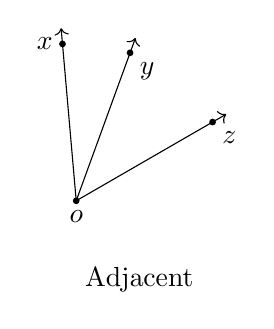
\begin{tikzpicture}[scale=2]
  \coordinate [label=below:\(o\)] (O) at (0:0);
  \coordinate [label=left:\(x\)] (X) at (95:1);
  \coordinate (X') at (95:1.1);
  \coordinate [label=below right:\(y\)] (Y) at (70:1);
  \coordinate (Y') at (70:1.1);
  \coordinate [label=below right:\(z\)] (Z) at (30:1);
  \coordinate (Z') at (30:1.1);

  \draw [fill] (O) circle [radius=0.5pt];
  \draw [fill] (X) circle [radius=0.5pt];
  \draw [fill] (Y) circle [radius=0.5pt];
  \draw [fill] (Z) circle [radius=0.5pt];

  \draw [->] (O) -- (X');
  \draw [->] (O) -- (Y');
  \draw [->] (O) -- (Z');

  \node at (0.4,-0.5) {Adjacent};
\end{tikzpicture}
\quad\quad
\begin{tikzpicture}[scale=2]
  \coordinate [label=below left:\(o\)] (O) at (0:0);
  \coordinate [label=below left:\(x\)] (X) at (170:0.7);
  \coordinate (X') at (170:0.8);
  \coordinate [label=below right:\(y\)] (Y) at (70:0.7);
  \coordinate (Y') at (70:0.8);
  \coordinate [label=below left:\(z\)] (Z) at (-10:0.7);
  \coordinate (Z') at (-10:0.8);

  \draw [fill] (O) circle [radius=0.5pt];
  \draw [fill] (X) circle [radius=0.5pt];
  \draw [fill] (Y) circle [radius=0.5pt];
  \draw [fill] (Z) circle [radius=0.5pt];

  \draw [->] (O) -- (X');
  \draw [->] (O) -- (Y');
  \draw [->] (O) -- (Z');

  \node at (0,-0.8) {Linear};
\end{tikzpicture}
\quad\quad
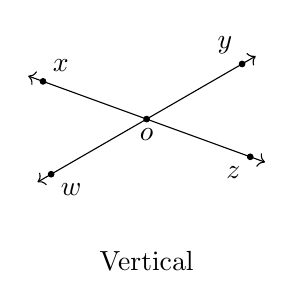
\begin{tikzpicture}[scale=2]
  \coordinate [label=below:\(o\)] (O) at (0:0);
  \coordinate [label=above right:\(x\)] (X) at (160:0.7);
  \coordinate (X') at (160:0.8);
  \coordinate [label=above left:\(y\)] (Y) at (30:0.7);
  \coordinate (Y') at (30:0.8);
  \coordinate [label=below left:\(z\)] (Z) at (-20:0.7);
  \coordinate (Z') at (-20:0.8);
  \coordinate [label=below right:\(w\)] (W) at (210:0.7);
  \coordinate (W') at (210:0.8);

  \draw [fill] (O) circle [radius=0.5pt];
  \draw [fill] (X) circle [radius=0.5pt];
  \draw [fill] (Y) circle [radius=0.5pt];
  \draw [fill] (Z) circle [radius=0.5pt];
  \draw [fill] (W) circle [radius=0.5pt];

  \draw [->] (O) -- (X');
  \draw [->] (O) -- (Y');
  \draw [->] (O) -- (Z');
  \draw [->] (O) -- (W');

  \node at (0,-0.9) {Vertical};
\end{tikzpicture}
\caption{\label{fig:angle-pairs}Some types of angle pairs.}
\end{center}
\end{figure}

\begin{thm}[Crossbar Theorem]
Suppose \(O\), \(A\), and \(B\) are noncollinear points in an ordered geometry, and that \(C \in \INTANGLE{A}{O}{B}\).
Then \(\RAY{O}{C}\) cuts \(\SEGMENT{A}{B}\) at a unique point \(D\).
(See \autoref{fig:crossbar-thm}.)
\end{thm}

\begin{figure}[h]
\begin{center}
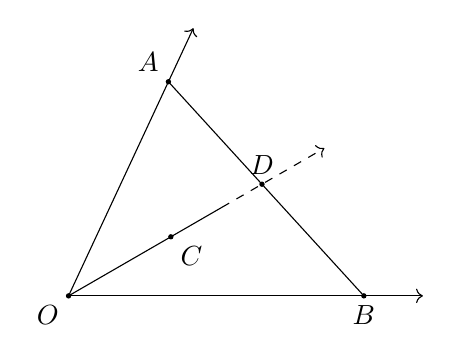
\begin{tikzpicture}[scale=1.5]
  \coordinate [label=below left:\(O\)] (O) at (0  : 0);
  \coordinate [label=above left:\(A\)] (A) at (65 : 2);
  \coordinate (A')  at (65 : 2.5);
  \coordinate [label=below:\(B\)]      (B) at (0  : 2.5);
  \coordinate (B')  at (0  : 3);
  \coordinate (C)   at (30 : 1);
  \coordinate (C')  at (30 : 1.5);
  \coordinate (C'') at (30 : 2.5);

  \coordinate [label=above:\(D\)] (D) at (intersection of A--B and O--C'');

  \draw [->] (O) -- (A');
  \draw [->] (O) -- (B');

  \draw [fill] (O) circle [radius=0.5pt];
  \draw [fill] (A) circle [radius=0.5pt];
  \draw [fill] (B) circle [radius=0.5pt];

  \draw (O) -- (C');
  \draw [dashed, ->] (C') -- (C'');

  \draw [fill] (C) circle [radius=0.5pt];
  \node [below right] at (C) {\(C\)};

  \draw (A) -- (B);

  \draw [fill] (D) circle [radius=0.5pt];
\end{tikzpicture}
\caption{\label{fig:crossbar-thm}The Crossbar Theorem}
\end{center}
\end{figure}

\begin{proof}
By the Interpolation property, there is a point \(P\) on \(\LINE{O}{A}\) such that \(\BETWEEN{P}{O}{A}\).
Note that \(A\) and \(P\) are on opposite sides of \(\LINE{O}{B}\), so that \(P\) and \(C\) are on opposite sides of \(\LINE{O}{B}\).
(Since \(A\) and \(C\) are on the same side of \(\LINE{O}{B}\) by definition.) Consider now the triangle \(\TRIANGLE{P}{A}{B}\).
Note that the line \(\LINE{O}{C}\) does not contain \(A\), \(B\), or \(P\), since \(C\) is not on \(\LINE{O}{A}\) or \(\LINE{O}{B}\) by hypothesis.
Moreover, \(\LINE{O}{C}\) cuts \(\SEGMENT{P}{A}\) at \(O\).
By Pasch's Axiom, \(\LINE{O}{C}\) must also cut either \(\SEGMENT{P}{B}\) or \(\SEGMENT{A}{B}\).

Suppose \(\LINE{O}{C}\) cuts \(\SEGMENT{P}{B}\) at a (necessarily unique) point \(Q\).
Note that \(\LINE{O}{C} = \LINE{Q}{C}\).
Now \(P\) and \(Q\) are on the same side of \(\LINE{O}{B}\), so that \(Q\) and \(C\) are on \emph{opposite} sides of \(\LINE{O}{B}\).
Thus, there is a unique point \(R\) on \(\LINE{O}{B}\) such that \(\BETWEEN{Q}{R}{C}\).
In particular, \(R \in \LINE{O}{C}\).
Now we have \(O,R \in \LINE{O}{C}\) and \(O, R \in \LINE{O}{B}\), so that \(\LINE{O}{C} = \LINE{O}{B}\), a contradiction.

Hence \(\LINE{O}{C}\) must cut \(\SEGMENT{A}{B}\) at a unique point; say \(D\).
Now \(D\) and \(A\) are on the same side of \(\LINE{O}{B}\), and so \(C\) and \(D\) are on the same side of \(\LINE{O}{B}\); in particular, we cannot have \(\BETWEEN{D}{O}{C}\).
So in fact \(\RAY{O}{C}\) cuts \(\SEGMENT{A}{B}\) at a unique point.
\end{proof}

\begin{dfn}[Angle Interior]
Suppose \(x\), \(o\), and \(y\) are noncollinear points in an ordered geometry.
Note that the lines \(\LINE{o}{x}\) and \(\LINE{o}{y}\) each divide \(P\) into half-planes.
Let \(H_1\) be the \(y\) half-plane of \(\LINE{o}{x}\), and let \(K_1\) be the \(x\) half-plane of \(\LINE{o}{y}\).
We define the \emph{interior}\index{interior!of an angle} of \(\ANGLE{x}{o}{y}\) to be the set \[ \INTANGLE{x}{o}{y} = H_1 \cap K_1. \]
If \(x\), \(y\), and \(o\) are collinear, then the interior of \(\ANGLE{x}{o}{y}\) is not defined.
\end{dfn}



\chapter{Neutral Plane Geometry}
\newpage

  \section{Congruence}
    Intuitively, we want to say that two sets of points in a geometry are ``congruent'' if they have the same size and shape.
But what exactly do ``size'' and ``shape'' mean?
Rather than defining congruence once and for all, we will instead define two primitive forms of congruence on segments and angles.
Then congruence for more complicated sets can be defined in terms of the primitives.

\begin{dfn}[Segment Congruence]
Let \(P\) be an ordered geometry, and suppose we have an equivalence relation on pairs of points, denoted \(\SEGCONG{\ast}{\ast}{\ast}{\ast}\).
We call \(\SEGCONG{\ast}{\ast}{\ast}{\ast}\) a \emph{segment congruence}\index{congruence!of segments} if the following properties are satisfied.
\begin{proplist}
\item[SC1.] \(\SEGCONG{x}{x}{y}{y}\) for all points \(x\) and \(y\).
\item[SC2.] \(\SEGCONG{x}{y}{y}{x}\) for all points \(x\) and \(y\).
\item[SC3.] If \(z \in \RAY{x}{y}\) such that \(\SEGCONG{x}{z}{x}{y}\), then \(z = y\).
\end{proplist}
In this case, \(\SEGCONG{\ast}{\ast}{\ast}{\ast}\) is well-defined on the set of \emph{segments} in \(P\), where we write \(\SEGMENT{x}{y} \equiv \SEGMENT{a}{b}\) to mean \(\SEGCONG{x}{y}{a}{b}\).
\end{dfn}

The first property handles the ``trivial'' case, the second makes the relation well-defined on segments, and the third ensures that it differentiates between segments on the same ray which share an endpoint.

\begin{dfn}[Angle Congruence]
Let \(P\) be an ordered geometry, and suppose we have an equivalence relation on triples of points, denoted \(\ANGCONG{\ast}{\ast}{\ast}{\ast}{\ast}{\ast}\).
We call \(\ANGCONG{\ast}{\ast}{\ast}{\ast}{\ast}{\ast}\) an \emph{angle congruence}\index{congruence!of angles} if the following properties are satisfied.
\begin{itemize}
\item[AC1.] If \(\BETWEEN{a_1}{b_1}{c_1}\) and \(\BETWEEN{a_2}{b_2}{c_2}\), then \(\ANGCONG{a_1}{b_1}{c_1}{a_2}{b_2}{c_2}\) and \(\ANGCONG{b_1}{a_1}{c_1}{b_2}{a_2}{c_2}\), and it is not the case that \(\ANGCONG{a_1}{b_1}{c_1}{b_1}{a_1}{c_1}\).
\item[AC2.] If \(a\), \(b\), \(o\), \(x\), and \(y\) are points such that \(o \notin \{a,b,x,y\}\), \(x \in \RAY{o}{a}\), and \(y \in \RAY{o}{b}\), then \(\ANGCONG{a}{o}{b}{x}{o}{y}\).
\item[AC3.] If \(a\), \(b\), and \(o\) are points such that \(o \notin \{a,b\}\), then \(\ANGCONG{a}{o}{b}{b}{o}{a}\).
\item[AC4.] If \(a\), \(b\), and \(o\) are distinct noncollinear points and \(x\) is on the \(b\)-side of \(\LINE{o}{a}\) such that \(\ANGCONG{a}{o}{b}{a}{o}{x}\), then \(x \in \RAY{o}{b}\).
\end{itemize}
In this case, \(\ANGCONG{\ast}{\ast}{\ast}{\ast}{\ast}{\ast}\) is an equivalence relation on the set of \emph{angles} in \(P\), and we write \(\ANGLE{a}{o}{b} \equiv \ANGLE{x}{p}{y}\) to mean \(\ANGCONG{a}{o}{b}{x}{p}{y}\).
\end{dfn}

Much like the properties of segment congruence, the first property handles the trivial cases, the second and third make the relation well-defined on angles, and the fourth ensures that it differentiates between angles on one half-plane which share a vertex.

\begin{dfn}[Congruence Geometry]
Let \(P\) be an ordered geometry.
If \(P\) has a segment congruence and an angle congruence, we say that \(P\) is an \emph{congruence geometry}\index{congruence geometry}.
\end{dfn}

We can define congruence of many different kinds of figures in terms of segment and angle congruence.
For instance...

\begin{dfn}[Triangle Congruence]
Let \(a\), \(b\), and \(c\) be distinct points, and let \(x\), \(y\), and \(z\) be distinct points.
We say that \(\TRIANGLE{a}{b}{c}\) is \emph{congruent}\index{congruence!of triangles} to \(\TRIANGLE{x}{y}{z}\), denoted \(\TRIANGLE{a}{b}{c} \equiv \TRIANGLE{x}{y}{z}\), if \[ \SEGMENT{a}{b} \equiv \SEGMENT{x}{y}, \quad \SEGMENT{b}{c} \equiv \SEGMENT{y}{z}, \quad \mathrm{and} \quad \SEGMENT{c}{a} \equiv \SEGMENT{z}{x} \] and \[ \ANGLE{a}{b}{c} \equiv \ANGLE{x}{y}{z}, \quad \ANGLE{b}{c}{a} \equiv \ANGLE{y}{z}{x}, \quad \mathrm{and} \quad \ANGLE{c}{a}{b} \equiv \ANGLE{z}{x}{y}. \]
\end{dfn}

\begin{dfn}
Let \(a\), \(b\), and \(c\) be distinct points.
\begin{proplist}
\item We say that the triangle \(\TRIANGLE{a}{b}{c}\) is \emph{equilateral}\index{equilateral} if \(\SEGMENT{a}{b} \equiv \SEGMENT{b}{c} \equiv \SEGMENT{c}{a}\).
\item We say that the triangle \(\TRIANGLE{a}{b}{c}\) is \emph{isoceles}\index{isoceles} if two of its sides are congruent to each other.
\end{proplist}
\end{dfn}


\begin{dfn}[Supplementary Angles]
We say that angles \(\ANGLE{a}{o}{b}\) and \(\ANGLE{x}{p}{y}\) are \emph{supplementary}\index{supplementary angles} if there is a linear pair, \(\ANGLE{u}{q}{v}\) and \(\ANGLE{v}{q}{w}\), such that \(\ANGLE{a}{o}{b} \equiv \ANGLE{u}{q}{v}\) and \(\ANGLE{x}{p}{y} \equiv \ANGLE{v}{q}{w}\).
In this case we say that \(\ANGLE{x}{p}{y}\) is a \emph{supplement} of \(\ANGLE{a}{o}{b}\).
\end{dfn}

\begin{prop}
Let \(P\) be a congruence geometry.
\begin{proplist}
\item If two angles form a linear pair, then they are supplementary.
\item Every angle has a supplement.
\end{proplist}
\end{prop}

\begin{dfn}
An angle is called \emph{right} if it is supplementary to itself.
\end{dfn}


%---------%
\Exercises%
%---------%

\begin{exercise}
Show that triangle congruence is an equivalence relation.
\end{exercise}

\begin{exercise}
Let \(\alpha\), \(\beta\), and \(\gamma\) be angles in a congruence geometry such that \(\alpha\) and \(\beta\) are supplementary and \(\beta \equiv \gamma\).
Show that \(\alpha\) and \(\gamma\) are supplementary.
\end{exercise}

    \newpage

  \section{Plane Geometry}
    \begin{dfn}[Plane Geometry]
Let \(P\) be an ordered geometry with a segment congruence and an angle congruence.
We say that \(P\) is a \emph{plane geometry} if the following properties are satisfied.
\begin{proplist}
\item[PG1.] \textbf{Right Angle Property.} Any two right angles are congruent.

\item[PG2.] \textbf{Angle-Side Congruence.} Suppose \(a_1\), \(b_1\), and \(c_1\) are distinct points and \(a_2\), \(b_2\), and \(c_2\) are distinct points such that \(\SEGMENT{b_1}{a_1} \equiv \SEGMENT{b_2}{a_2}\) and \(\SEGMENT{b_1}{c_1} \equiv \SEGMENT{b_2}{c_2}\).
Then \(\SEGMENT{a_1}{c_1} \equiv \SEGMENT{a_2}{c_2}\) if and only if \(\ANGLE{a_1}{b_1}{c_1} \equiv \ANGLE{a_2}{b_2}{c_2}\).

\item[PG3.] \textbf{Circle Cut.} If \(o\), \(a\), and \(b\) are points such that \(a \neq o\) and \(b \neq o\), then there is a point \(c \in \RAY{o}{b}\) such that \(\SEGMENT{o}{c} \equiv \SEGMENT{o}{a}\).

\begin{center}
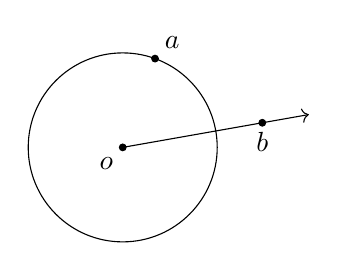
\begin{tikzpicture}[scale=0.6]
  \coordinate [label=below left:\(o\)]  (o) at (0  : 0);
  \draw [fill] (o) circle [radius=2pt];
  \coordinate [label=above right:\(a\)] (a) at (70 : 2);
  \draw [fill] (a) circle [radius=2pt];
  \coordinate [label=below:\(b\)]       (b) at (10 : 3);
  \draw [fill] (b) circle [radius=2pt];
  \draw [->] (o) -- (10: 4);
  \draw (o) circle [radius=2];
\end{tikzpicture}
\end{center}

\item[PG4.] \textbf{Interleaved Diameters.} Let \(C_1\) and \(C_2\) be circles centered at distinct points \(o_1\) and \(o_2\), respectively.
Further suppose we have diameters \(\SEGMENT{a_1}{b_1}\) of \(C_1\) and \(\SEGMENT{a_2}{b_2}\) of \(C_2\) such that \(\BETWEEN{a_1}{o_1}{a_2}\) and \(\BETWEEN{a_1}{o_2}{a_2}\).
Then \(C_1 \cap C_2\) is nonempty if and only if \(\BETWEENS{a_1b_2b_1a_2}\), and in this case \(C_1 \cap C_2\) consists of exactly two points which are on opposite sides of \(\LINE{o_1}{o_2}\).

\begin{center}
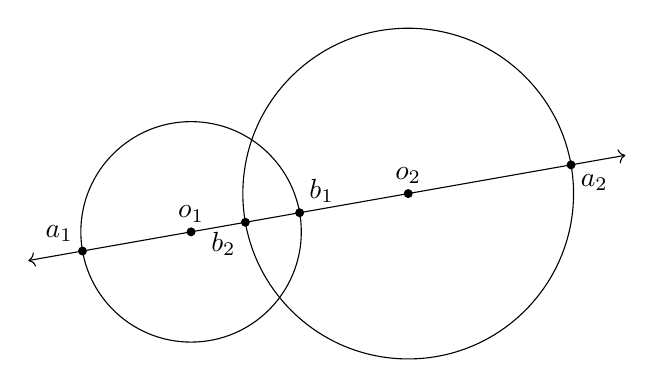
\begin{tikzpicture}[scale=0.7]
  \coordinate [label=above:{\(o_1\)}]  (o1) at (0,0);
  \draw [fill] (o1) circle [radius=2pt];
  \coordinate [label=above left:{\(a_1\)}] (a1) at ($ (o1)+(10 : -2) $);
  \draw [fill] (a1) circle [radius=2pt];
  \coordinate [label=above right:{\(b_1\)}] (b1) at ($ (o1)+(10 : 2) $);
  \draw [fill] (b1) circle [radius=2pt];
  \draw (o1) circle [radius=2];
  \coordinate [label=above:\(o_2\)]  (o2) at ($ (o1)+(10 : 4) $);
  \draw [fill] (o2) circle [radius=2pt];
  \coordinate [label=below right:\(a_2\)] (a2) at ($ (o2)+(10 : 3) $);
  \draw [fill] (a2) circle [radius=2pt];
  \coordinate [label=below left:\(b_2\)] (b2) at ($ (o2)+(10 : -3) $);
  \draw [fill] (b2) circle [radius=2pt];
  \draw (o2) circle [radius=3];
  \draw [<->] ($ (o1)+(10 : -3) $) -- ($ (o2)+(10 : 4) $);
\end{tikzpicture}
\end{center}
\end{proplist}
\end{dfn}

Each of these properties says something which is (hopefully!) fairly intuitive.
Angle-Side Congruence provides an essential link between segment congruence and angle congruence, which are otherwise unrelated.
The Circle Cut and Interleaved Diameters properties allow us to construct points on the intersection of a circle with a central ray and of two circles, respectively.
(Without these we have no way to construct points on circles!)

We finally have enough technology to start doing some more recognizable geometry.
For the remainder of this chapter \(P\) is a plane geometry.
First, we give two shortcut results for determining when two triangles are congruent.

\begin{prop}[SSS Theorem]\label{prop:sss-theorem}
If two nondegenerate triangles can be labeled such that corresponding sides are congruent, then the triangles are congruent.

More precisely, let \(a_1\), \(b_1\), and \(c_1\) be distinct points and \(a_2\), \(b_2\), and \(c_2\) be distinct points.
If \(\SEGMENT{a_1}{b_1} \equiv \SEGMENT{a_2}{b_2}\), \(\SEGMENT{b_1}{c_1} \equiv \SEGMENT{b_2}{c_2}\), and \(\SEGMENT{c_1}{a_1} \equiv \SEGMENT{c_2}{a_2}\), then \(\TRIANGLE{a_1}{b_1}{c_1} \equiv \TRIANGLE{a_2}{b_2}{c_2}\).
\end{prop}

\begin{proof}
We have \(\ANGLE{a_1}{b_1}{c_1} \equiv \ANGLE{a_2}{b_2}{c_2}\), \(\ANGLE{b_1}{c_1}{a_1} \equiv \ANGLE{b_2}{c_2}{a_2}\), and \(\ANGLE{c_1}{a_1}{b_1} \equiv \ANGLE{c_2}{a_2}{b_2}\) using the Angle-Side Congruence property three times.
\end{proof}

\begin{prop}[SAS Theorem]\label{prop:sas-theorem}
If two nondegenerate triangles can be labeled such that two corresponding sides, and the angles between, are congruent, then the triangles are congruent.

More precisely, let \(a_1\), \(b_1\), and \(c_1\) be distinct points, and \(a_2\), \(b_2\), and \(c_2\) be distinct points.
If \(\SEGMENT{a_1}{b_1} \equiv \SEGMENT{a_2}{b_2}\), \(\SEGMENT{b_1}{c_1} \equiv \SEGMENT{b_2}{c_2}\), and \(\ANGLE{a_1}{b_1}{c_1} \equiv \ANGLE{a_2}{b_2}{c_2}\), then \(\TRIANGLE{a_1}{b_1}{c_1} \equiv \TRIANGLE{a_2}{b_2}{c_2}\).
\end{prop}

\begin{proof}
We have \(\SEGMENT{a_1}{c_1} \equiv \SEGMENT{a_2}{c_2}\) by Angle-Side Congruence, and then \hyperref[prop:sss-theorem]{SSS} applies.
\end{proof}

\begin{cor}[Pons Asinorum]\label{cor:pons-asinorum}
If \(\TRIANGLE{a}{b}{c}\) is isoceles with \(\SEGMENT{a}{b} \equiv \SEGMENT{b}{c}\), then \(\ANGLE{b}{a}{c} \equiv \ANGLE{b}{c}{a}\).
\end{cor}

\begin{proof}
We have two triangles, \(\TRIANGLE{b}{a}{c}\) and \(\TRIANGLE{b}{c}{a}\), such that \(\SEGMENT{b}{c}\equiv \SEGMENT{b}{a}\), \(\SEGMENT{b}{a} \equiv \SEGMENT{b}{c}\), and \(\ANGLE{c}{b}{a} \equiv \SEGMENT{a}{b}{c}\).
By \hyperref[prop:sas-theorem]{SAS} we have \(\TRIANGLE{b}{a}{c} \equiv \TRIANGLE{b}{c}{a}\), and thus \(\ANGLE{b}{a}{c} \equiv \ANGLE{b}{c}{a}\) as needed.
\end{proof}

\begin{cor}
Every triangle which is equilateral is also equiangular; all three interior angles are congruent.
\end{cor}

\begin{proof}
Follows from two applications of Pons Asinorum.
\end{proof}

\begin{cor}[Segment Addition]\label{cor:segment-addition}
Suppose \(\BETWEEN{a_1}{b_1}{c_1}\) and \(\BETWEEN{a_2}{b_2}{c_2}\).
If any two of \(\SEGMENT{a_1}{b_1} \equiv \SEGMENT{a_2}{b_2}\), \(\SEGMENT{b_1}{c_1} \equiv \SEGMENT{b_2}{c_2}\), and \(\SEGMENT{a_1}{c_1} \equiv \SEGMENT{a_2}{c_2}\) hold, then so does the third.
\end{cor}

\begin{proof}
Note that \(\ANGLE{a_1}{b_1}{c_1} \equiv \ANGLE{a_2}{b_2}{c_2}\), \(\ANGLE{b_1}{c_1}{a_1} \equiv \ANGLE{b_2}{c_2}{a_2}\), and \(\ANGLE{c_1}{a_1}{b_1} \equiv \ANGLE{c_2}{a_2}{b_2}\) by AC1.
The result then follows from three applications of \hyperref[prop:sas-theorem]{SAS}.
\end{proof}

\begin{dfn}[Antipode]
Let \(a\), \(b\), and \(c\) be points.
We say that \(c\) is an \emph{antipode}\index{antipode} of \(a\) \emph{through} \(b\) if \(\BETWEEN{a}{b}{c}\) and \(\SEGMENT{a}{b} \equiv \SEGMENT{b}{c}\).
\end{dfn}

\begin{construct}[Antipode]\label{construct:antipode}
Given distinct points \(a\) and \(b\), there is a unique point \(c\) such that \(c\) is an antipode of \(a\) through \(b\).
\end{construct}

\begin{proof}
First we show existence.
Using the Interpolation property, there is a point \(u\) such that \(\BETWEEN{u}{b}{a}\).
Now using Circle Cut, there is a point \(c \in \RAY{b}{u} \cap \CIRCLE{b}{a}\).
Note that \(\BETWEEN{a}{b}{c}\), and we have \(\SEGMENT{b}{c} \equiv \SEGMENT{b}{a}\) as needed.
Next we show uniqueness.
Suppose \(d\) is a point such that \(\BETWEEN{a}{b}{d}\) and \(\SEGMENT{a}{b} \equiv \SEGMENT{b}{d}\).
But then \(d \in \RAY{b}{c}\), and in fact \(c = d\) by AC4.
\end{proof}

\begin{construct}[Equilateral triangle with a given side]\label{construct:equilateral-points}
Given distinct points \(a\) and \(b\), there exist points \(c_1\) and \(c_2\), on opposite sides of \(\LINE{a}{b}\), such that \(\TRIANGLE{a}{b}{c_1}\) and \(\TRIANGLE{a}{b}{c_2}\) are equilateral.
In fact, we have \(\TRIANGLE{a}{b}{c_1} \equiv \TRIANGLE{a}{b}{c_2}\).
\end{construct}

\begin{proof}
First, construct the antipode \(h\) of \(b\) through \(a\), and construct the antipode \(k\) of \(a\) through \(b\).
Note that \(\BETWEENS{habk}\), and that \(\SEGMENT{a}{h} \equiv \SEGMENT{a}{b}\) and \(\SEGMENT{b}{k} \equiv \SEGMENT{b}{a}\); that is, \(a\) is a midpoint of \(\SEGMENT{h}{b}\) and \(b\) a midpoint of \(\SEGMENT{a}{k}\), so that \(a\) is the center of \(\CIRCLE{a}{b}\) with diameter \(\SEGMENT{h}{b}\) and \(b\) is the center of \(\CIRCLE{b}{a}\) with diameter \(\SEGMENT{a}{k}\).
Thus the Interleaved Diameters property applies, and we have two points \(c_1,c_2 \in \CIRCLE{a}{b} \cap \CIRCLE{b}{a}\) which are in opposite halfplanes of \(\LINE{a}{b}\).
Note that \(\SEGMENT{a}{c_1} \equiv \SEGMENT{a}{b} \equiv \SEGMENT{b}{c_1}\), and thus \(\TRIANGLE{a}{b}{c_1}\) is equilateral.
Similarly, \(\TRIANGLE{a}{b}{c_2}\) is equilateral.
Moreover, we see that \(\TRIANGLE{a}{b}{c_1} \equiv \TRIANGLE{a}{b}{c_2}\) by the SSS Theorem.
\end{proof}

\begin{lem}[Betweenness Transfer]\label{lem:betweenness-transfer}
Let \(a_1\), \(b_1\), \(c_1\), \(a_2\), \(b_2\), and \(c_2\) be points such that \(\BETWEEN{a_1}{b_1}{c_1}\), \(b_2 \in \RAY{a_2}{c_2}\), \(\SEGMENT{a_1}{b_1} \equiv \SEGMENT{a_2}{b_2}\), and \(\SEGMENT{a_1}{c_1} \equiv \SEGMENT{a_2}{c_2}\).
Then \(\BETWEEN{a_2}{b_2}{c_2}\).
\end{lem}

\begin{proof}
Note that \(a_1\), \(b_1\), and \(c_1\) are distinct.
Since \(\SEGMENT{a_1}{b_1} \equiv \SEGMENT{a_2}{b_2}\), \(a_2\) and \(b_2\) are distinct.
If \(b_2 = c_2\), then we have \(\SEGMENT{a_1}{b_1} \equiv \SEGMENT{a_1}{c_1}\), so that \(b_1 = c_1\) by S3 -- a contradiction.
So \(b_2\) and \(c_2\) are distinct.
Because \(b_2 \in \RAY{a_2}{c_2}\), there are two possibilities: either \(\BETWEEN{a_2}{c_2}{b_2}\) or \(\BETWEEN{a_2}{b_2}{c_2}\).

Suppose \(\BETWEEN{a_2}{c_2}{b_2}\).
Now \(\ANGLE{c_2}{a_2}{b_2} \equiv \ANGLE{c_1}{a_1}{b_1}\) (both angles are flat), and by \hyperref[prop:sas-theorem]{SAS} we have \(\TRIANGLE{c_1}{a_1}{b_1} \equiv \TRIANGLE{c_2}{a_2}{b_2}\).
In particular, we have \(\ANGLE{a_1}{b_1}{c_1} \equiv \ANGLE{a_2}{b_2}{c_2}\); a contradiction, as in this case \(\ANGLE{a_1}{b_1}{c_1}\) is straight while \(\ANGLE{a_2}{b_2}{c_2}\) is flat.
Thus \(\BETWEEN{a_2}{b_2}{c_2}\) as claimed.
\end{proof}

\begin{construct}[Segment Copy Theorem]
Let \(a\) and \(b\) be distinct points, and let \(o\) and \(t\) be distinct points.
Then there is a unique point \(x\) on \(\RAY{o}{t}\) such that \(\SEGMENT{o}{x} \equiv \SEGMENT{a}{b}\).
\end{construct}

\begin{proof}
First we construct a point \(z\) such that \(\TRIANGLE{a}{o}{z}\) is equilateral; now \(\SEGMENT{z}{a} \equiv \SEGMENT{z}{o}\).
Using the Interpolation property, construct a point \(h\) such that \(\BETWEEN{z}{a}{h}\), and using the Circle Cut property, construct a point \(u\) on \(\RAY{a}{h}\) such that \(\SEGMENT{a}{u} \equiv \SEGMENT{a}{b}\).
Again using Circle Cut, construct a point \(v\) on \(\RAY{z}{o}\) such that \(\SEGMENT{z}{v} \equiv \SEGMENT{z}{u}\).
By \lemref{lem:betweenness-transfer} we have \(\BETWEEN{z}{o}{v}\).
Now \(\SEGMENT{z}{a} \equiv \SEGMENT{z}{o}\) and \(\SEGMENT{z}{u} \equiv \SEGMENT{z}{v}\), thus \(\SEGMENT{a}{u} \equiv \SEGMENT{o}{v}\).
Again using Circle Cut, construct a point \(x\) on \(\RAY{o}{t}\) such that \(\SEGMENT{o}{x} \equiv \SEGMENT{o}{v}\).
Then we have \(\SEGMENT{o}{x} \equiv \SEGMENT{o}{v} \equiv \SEGMENT{a}{u} \equiv \SEGMENT{a}{b}\) as needed.
Uniqueness follows from SC3.
\end{proof}

\begin{construct}[Angle Copy Theorem]
Let \(a\), \(o\), \(b\) be distinct noncollinear points and let \(p\) and \(x\) be distinct points.
There exist two points \(y_1\) and \(y_2\), on opposite sides of \(\LINE{p}{x}\), such that \(\ANGLE{x}{p}{y_1} \equiv \ANGLE{x}{p}{y_2} \equiv \ANGLE{a}{o}{b}\). 
\end{construct}

\begin{proof}
First copy segment \(\SEGMENT{o}{b}\) onto \(\RAY{p}{x}\) at the point \(u\), then copy the segment \(\SEGMENT{b}{a}\) onto the ray \(\RAY{u}{p}\) at the point \(v\).
Now copy \(\SEGMENT{o}{a}\) onto \(\RAY{p}{x}\) at the point \(w\).
Note that \(\SEGMENT{o}{a} \equiv \SEGMENT{p}{w}\), \(\SEGMENT{o}{b} \equiv \SEGMENT{p}{u}\), and \(\SEGMENT{b}{a} \equiv \SEGMENT{u}{v}\).
Moreover, the intersection \(\CIRCLE{o}{a} \cap \CIRCLE{b}{a}\) is nonempty, as it contains \(a\).
By the Interleaved Diameters property, \(\CIRCLE{p}{w} \cap \CIRCLE{u}{v}\) contains two points \(z_1\) and \(z_2\) on opposite sides of \(\LINE{p}{x}\).
By the SSS Theorem, we have \(\TRIANGLE{p}{u}{z_1} \equiv \TRIANGLE{o}{b}{a} \equiv \TRIANGLE{p}{u}{z_2}\), and thus \(\ANGLE{u}{p}{z_1} \equiv \ANGLE{a}{o}{b} \equiv \ANGLE{u}{p}{z_2}\) as needed.
\end{proof}

\begin{prop}[ASA Theorem]
Let \(a_1\), \(b_1\), and \(c_1\) be distinct noncollinear points, and let \(a_2\), \(b_2\), and \(c_2\) be distinct points.
If \(\ANGLE{a_1}{b_1}{c_1} \equiv \ANGLE{a_2}{b_2}{c_2}\), \(\SEGMENT{b_1}{c_1} \equiv \SEGMENT{b_2}{c_2}\), and \(\ANGLE{b_1}{c_1}{a_1} \equiv \ANGLE{b_2}{c_2}{a_2}\), then \(\TRIANGLE{a_1}{b_1}{c_1} \equiv \TRIANGLE{a_2}{b_2}{c_2}\).
\end{prop}

\begin{proof}
Copy \(\SEGMENT{b_2}{a_2}\) onto \(\RAY{b_1}{a_1}\) at \(d\).
Note that \(d\) and \(a_1\) are on the same side of \(\LINE{b_1}{c_1}\).
Moreover, we have \(\TRIANGLE{d}{b_1}{c_1} \equiv \TRIANGLE{a_2}{b_2}{c_2}\) by \hyperref[prop:sas-theorem]{SAS}, and so \(\ANGLE{b_1}{c_1}{d} \equiv \ANGLE{b_2}{c_2}{a_2} \equiv \ANGLE{b_1}{c_1}{a_1}\).
By AC4, we have \(d \in \RAY{c_1}{a_1}\).
Now \(d\) is on both \(\LINE{b_1}{a_1}\) and \(\LINE{c_1}{a_1}\), and since \(a_1\), \(b_1\), and \(c_1\) are not collinear, we must have \(d = a_1\).
So we have \(\TRIANGLE{a_1}{b_1}{c_1} \equiv \TRIANGLE{a_2}{b_2}{c_2}\) as claimed.
\end{proof}

    \newpage

  \section{Transversals}
    \begin{prop}[Supplements are unique] \mbox{}
\begin{proplist}
\item Suppose that \(\ANGLE{a_1}{o_1}{b_1}\) and \(\ANGLE{b_1}{o_1}{c_1}\) are a linear pair, and that \(\ANGLE{a_2}{o_2}{b_2}\) and \(\ANGLE{b_2}{o_2}{c_2}\) are a linear pair.
If \(\ANGLE{a_1}{o_1}{b_1} \equiv \ANGLE{a_2}{o_2}{b_2}\), then \(\ANGLE{b_1}{o_1}{c_1} \equiv \ANGLE{b_2}{o_2}{c_2}\).

\begin{center}
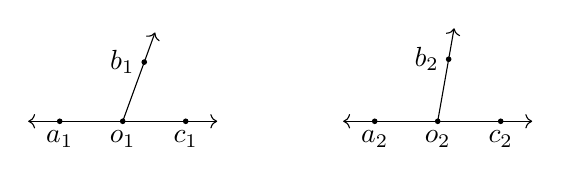
\begin{tikzpicture}[scale=0.8]
  \coordinate [label=below:\(o_1\)] (o1) at (-3,0);
  \coordinate [label=below:\(a_1\)] (a1) at ($ (o1)+(180:1) $);
  \coordinate [label=left:\(b_1\)] (b1) at ($ (o1)+(70:1) $);
  \coordinate [label=below:\(c_1\)] (c1) at ($ (o1)+(0:1) $);

  \draw [fill] (o1) circle [radius=1pt];
  \draw [fill] (a1) circle [radius=1pt];
  \draw [fill] (b1) circle [radius=1pt];
  \draw [fill] (c1) circle [radius=1pt];

  \draw [->] (o1) -- ($ (a1)+(180:0.5) $);
  \draw [->] (o1) -- ($ (b1)+(70:0.5) $);
  \draw [->] (o1) -- ($ (c1)+(0:0.5) $);

  \coordinate [label=below:\(o_2\)] (o2) at (2,0);
  \coordinate [label=below:\(a_2\)] (a2) at ($ (o2)+(180:1) $);
  \coordinate [label=left:\(b_2\)] (b2) at ($ (o2)+(80:1) $);
  \coordinate [label=below:\(c_2\)] (c2) at ($ (o2)+(0:1) $);

  \draw [fill] (o2) circle [radius=1pt];
  \draw [fill] (a2) circle [radius=1pt];
  \draw [fill] (b2) circle [radius=1pt];
  \draw [fill] (c2) circle [radius=1pt];

  \draw [->] (o2) -- ($ (a2)+(180:0.5) $);
  \draw [->] (o2) -- ($ (b2)+(80:0.5) $);
  \draw [->] (o2) -- ($ (c2)+(0:0.5) $);
\end{tikzpicture}
\end{center}

\item Suppose \(\alpha\), \(\beta\), and \(\gamma\) are angles such that \(\alpha\) and \(\beta\) are supplementary and \(\alpha\) and \(\gamma\) are supplementary.
Then \(\alpha \equiv \gamma\).
\end{proplist}
\end{prop}

\begin{proof}\mbox{}
\begin{proplist}
\item Suppose we have two such linear pairs.
Without loss of generality, we can suppose that \[ \SEGMENT{o_1}{a_1} \equiv \SEGMENT{o_1}{b_1} \equiv \SEGMENT{o_1}{c_1} \equiv \SEGMENT{o_2}{a_2} \equiv \SEGMENT{o_2}{b_2} \equiv \SEGMENT{o_2}{c_2}. \] (If they aren't, we can use Circle Cut and the Segment Copy construction to find such points.) Now \(\TRIANGLE{b_1}{o_1}{a_1} \equiv \TRIANGLE{b_2}{o_2}{a_2}\) by SAS, so that \(\ANGLE{b_1}{a_1}{o_1} \equiv \ANGLE{b_2}{a_2}{o_2}\).
Now \(\SEGMENT{a_1}{c_1} \equiv \SEGMENT{a_2}{c_2}\), so that \(\TRIANGLE{b_1}{a_1}{c_1} \equiv \TRIANGLE{b_2}{a_2}{c_2}\) by SAS.
So \(\SEGMENT{b_1}{c_1} \equiv \SEGMENT{b_2}{c_2}\), and thus \(\TRIANGLE{b_1}{o_1}{c_1} \equiv \TRIANGLE{b_2}{o_2}{c_2}\) by SSS.
Thus \(\ANGLE{b_1}{o_1}{c_1} \equiv \ANGLE{b_2}{o_2}{c_2}\) as needed.

\item Follows from the definition of supplementary.
\qedhere
\end{proplist}
\end{proof}

\begin{cor}
If angles \(\alpha\) and \(\beta\) are a vertical pair, then \(\alpha \equiv \beta\).
\end{cor}

\begin{proof}
If \(\ANGLE{a}{o}{b}\) and \(\ANGLE{c}{o}{d}\) are a vertical pair, with \(\BETWEEN{b}{o}{c}\) and \(\BETWEEN{a}{o}{d}\), then both \(\ANGLE{a}{o}{b}\) and \(\ANGLE{c}{o}{d}\) are supplementary to \(\ANGLE{a}{o}{c}\).
\end{proof}

\begin{dfn}
An angle is called \emph{right} if it is supplementary to itself.
\end{dfn}

\begin{cor}
Any two right angles are congruent.
\end{cor}

\begin{proof}
Suppose angles \(\alpha\) and \(\beta\) are right.
We can copy \(\beta\) to an angle \(\beta'\) in the configuration of \ref{lem:coinitial-right-angle-congruence}.
Since supplements are congruent, \ref{lem:coinitial-right-angle-congruence} applies.
\end{proof}


\begin{dfn}[Transversal]
Suppose we have three lines \(\ell_1\), \(\ell_2\), and \(t\) in a plane geometry.
We say that \(t\) is a \emph{transversal}\index{transversal} of \(\ell_1\) and \(\ell_2\) if \(t\) cuts both \(\ell_1\) and \(\ell_2\) at unique points, and these points are distinct.

Suppose \(t\) is a transversal of \(\ell_1\) and \(\ell_2\), cutting these lines at \(o_1\) and \(o_2\), respectively as shown.

\begin{center}
\begin{tikzpicture}[scale=0.5]
  \coordinate (x1) at (-5,0);
  \coordinate (y1) at (4,0);
  \draw [<->] (x1) -- (y1);
  \node at (4,-0.5) {\(\ell_1\)};
  \coordinate (x2) at (-4,5);
  \coordinate (y2) at (4,3);
  \draw [<->] (x2) -- (y2);
  \node  at (-3,5.5) {\(\ell_2\)};
  \coordinate (x3) at (-1,-1);
  \coordinate (y3) at (1,6);
  \draw [<->] (x3) -- (y3);
  \node at (0.7,6) {\(t\)};
  \coordinate [label=below right:\(o_1\)] (o1) at (intersection of x1--y1 and x3--y3);
  \draw [fill] (o1) circle [radius=1pt];
  \coordinate [label=below left:\(o_2\)] (o2) at (intersection of x2--y2 and x3--y3);
  \draw [fill] (o2) circle [radius=1pt];
  \coordinate (x4) at (-0.5,2);
  \coordinate (y4) at (1,3);
  \coordinate [label=below:\(a\)] (a) at (intersection of x1--y1 and x4--y4);
  \draw [fill] (a) circle [radius=1pt];
  \coordinate [label=below:\(b\)] (b) at (intersection of x2--y2 and x4--y4);
  \draw [fill] (b) circle [radius=1pt];
\end{tikzpicture}
\end{center}

If \(a\) is on \(\ell_1\) and \(b\) is on \(\ell_2\) such that \(a\) and \(b\) are on opposite sides of \(t\), then we say that \(\ANGLE{a}{o_1}{o_2}\) and \(\ANGLE{b}{o_2}{o_1}\) are \emph{alternate interior angles}\index{alternate interior angles} of this transversal.
\end{dfn}

Every transversal has two pairs of alternate interior angles.

\begin{prop}[AIA Theorem]\label{prop:aia-theorem}
If two lines \(\ell_1\) and \(\ell_2\) are cut by a transversal \(t\) so that a pair of alternate interior angles are congruent, then \(\ell_1\) and \(\ell_2\) are parallel.
\end{prop}

\begin{proof}
Suppose \(t\) meets \(\ell_1\) and \(\ell_2\) at points \(o_1\) and \(o_2\) respectively, and that \(a\) and \(b\) are on \(\ell_1\) and \(\ell_2\), respectively, and on opposite sides of \(t\), such that \(\ANGLE{a}{o_1}{o_2} \equiv \ANGLE{b}{o_2}{o_1}\).
Now suppose by way of contradiction that \(\ell_1\) and \(\ell_2\) are \emph{not} parallel; rather, they meet at a point \(x\) which (WLOG) is on the \(a\)-side of \(t\).
Let \(c\) be on \(\ell_1\) such that \(\BETWEEN{a}{o_1}{c}\).
Copy \(\SEGMENT{o_1}{x}\) onto \(\RAY{o_2}{b}\) at the point \(y\).
Note that \(\SEGMENT{o_1}{x} \equiv \SEGMENT{o_2}{y}\), \(\SEGMENT{o_1}{o_2} \equiv \SEGMENT{o_2}{o_1}\), and \(\ANGLE{x}{o_1}{o_2} \equiv \ANGLE{y}{o_2}{o_1}\); by \hyperref[prop:sas-theorem]{SAS} we thus have \(\TRIANGLE{x}{o_1}{o_2} \equiv \TRIANGLE{y}{o_2}{o_1}\).
In particular, \(\ANGLE{o_2}{o_1}{y} \equiv \ANGLE{o_1}{o_2}{x}\).

\begin{center}
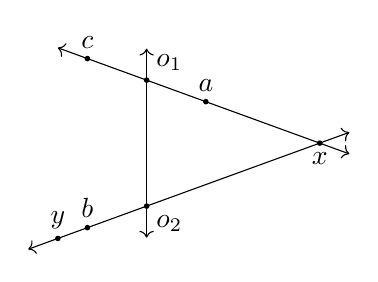
\begin{tikzpicture}[scale=0.8]
  \coordinate [label=above right:\(o_1\)] (o1) at (0,2);
  \coordinate [label=below right:\(o_2\)] (o2) at ($ (o1)+(270:2) $);
  \coordinate [label=above:\(a\)] (a) at ($ (o1)+(160:-1) $);
  \coordinate [label=above:\(c\)] (c) at ($ (o1)+(160:1) $);
  \coordinate [label=above:\(b\)] (b) at ($ (o2)+(200:1) $);
  \coordinate [label=below:\(x\)] (x) at (intersection of o1--a and o2--b);
  \coordinate [label=above:\(y\)] (y) at ($ (o2)+(200:1.5) $);

  \draw [fill] (o1) circle [radius=1pt];
  \draw [fill] (o2) circle [radius=1pt];
  \draw [fill] (a) circle [radius=1pt];
  \draw [fill] (c) circle [radius=1pt];
  \draw [fill] (b) circle [radius=1pt];
  \draw [fill] (x) circle [radius=1pt];
  \draw [fill] (y) circle [radius=1pt];

  \draw [<->] ($ (o1)+(90:0.5) $) -- ($ (o2)+(270:0.5) $);
  \draw [<->] ($ (y)+(200:0.5) $) -- ($ (x)+(200:-0.5) $);
  \draw [<->] ($ (c)+(160:0.5) $) -- ($ (x)+(160:-0.5) $);
\end{tikzpicture}
\end{center}

Note that \(\ANGLE{x}{o_2}{o_1}\) and \(\ANGLE{o_1}{o_2}{y}\) are supplementary, and \(\ANGLE{o_1}{o_2}{y} \equiv \ANGLE{a}{o_1}{o_2}\) by hypothesis, so that \(\ANGLE{a}{o_1}{o_2}\) and \(\ANGLE{x}{o_2}{o_1}\) are supplementary.
Since \(\ANGLE{x}{o_2}{o_1} \equiv \ANGLE{y}{o_1}{o_2}\), we have that \(\ANGLE{a}{o_1}{o_2}\) and \(\ANGLE{y}{o_1}{o_2}\) are supplementary.
But also \(\ANGLE{a}{o_1}{o_2}\) and \(\ANGLE{o_2}{o_1}{c}\) are supplementary.
Thus \(\ANGLE{o_2}{o_1}{y} \equiv \ANGLE{o_2}{o_1}{c}\).
By AC4, we have that \(o_1\), \(c\), and \(y\) are collinear, so that \(y \in \ell_1\).
But now \(\ell_1\) and \(\ell_2\) have two points in common -- \(x\) and \(y\) -- which are necessarily distinct as they are on opposite halfplanes of \(t\).
So we have \(\ell_1 = \ell_2\), a contradiction.

Thus \(\ell_1\) and \(\ell_2\) must be parallel. 
\end{proof}

\begin{cor}\label{cor:a-triangle-has-at-most-one-right-angle}
A triangle formed by three distinct noncollinear points cannot have two interior angles which are both right.
\end{cor}

\begin{proof}
Such a triangle would violate the \hyperref[prop:aia-theorem]{AIA Theorem} since right angles are self-supplementary, and any two right angles are congruent.
\end{proof}

\begin{prop}[AAS Theorem]\label{prop:aas-theorem}
Suppose we have distinct noncollinear points \(a_1\), \(b_1\), and \(c_1\) and distinct noncollinear points \(a_2\), \(b_2\), and \(c_2\) such that \(\ANGLE{c_1}{a_1}{b_1} \equiv \ANGLE{c_2}{a_2}{b_2}\), \(\ANGLE{a_1}{b_1}{c_1} \equiv \ANGLE{a_2}{b_2}{c_2}\), and \(\SEGMENT{b_1}{c_1} \equiv \SEGMENT{b_2}{c_2}\).
Then \(\TRIANGLE{a_1}{b_1}{c_1} \equiv \TRIANGLE{a_2}{b_2}{c_2}\).
\end{prop}

\begin{proof}
Copy \(\SEGMENT{b_1}{a_1}\) onto \(\RAY{b_2}{a_2}\) at the point \(w\).
Note that \(w \neq b_2\), since \(a_1 \neq b_1\).
Note also that \(\TRIANGLE{w}{b_2}{c_2} \equiv \TRIANGLE{a_1}{b_2}{c_2}\) by \hyperref[prop:sas-theorem]{SAS}, so that \(\ANGLE{b_1}{a_1}{c_1} \equiv \ANGLE{b_2}{w}{c_2}\).
Suppose now that \(w\) and \(a_2\) are distinct points; say \(\BETWEEN{b_2}{w}{a_2}\).
(The case \(\BETWEEN{b_2}{a_2}{w}\) is very similar.)
In this case \(\LINE{a_2}{c_2}\) and \(\LINE{w}{c_2}\) are lines cut by a transversal \(\LINE{a_2}{b_2}\).

\begin{center}
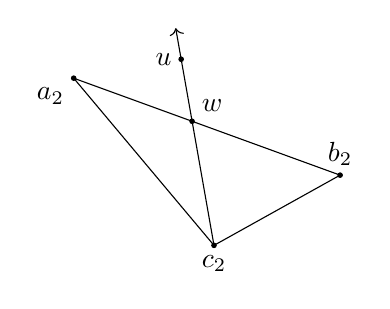
\begin{tikzpicture}[scale=0.8]
  \coordinate [label=above right:\(w\)] (w) at (0,0);
  \coordinate [label=below left:\(a_2\)] (a2) at ($ (w)+(160:2) $);
  \coordinate [label=above:\(b_2\)] (b2) at ($ (w)+(160:-2.5) $);
  \coordinate [label=below:\(c_2\)] (c2) at ($ (w)+(100:-2) $);
  \coordinate [label=left:\(u\)] (u) at ($ (w)+(100:1) $);

  \draw [fill] (w) circle [radius=1pt];
  \draw [fill] (a2) circle [radius=1pt];
  \draw [fill] (b2) circle [radius=1pt];
  \draw [fill] (c2) circle [radius=1pt];
  \draw [fill] (u) circle [radius=1pt];

  \draw (a2) -- (b2) -- (c2) -- cycle;
  \draw [->] (c2) -- ($ (u)+(100:0.5) $);
\end{tikzpicture}
\end{center}

Moreover, if we let \(u\) be a point such that \(\BETWEEN{u}{w}{c_2}\), then \(\ANGLE{u}{w}{a_2}\) and \(\ANGLE{b_2}{w}{c_2}\) are vertical, hence congruent, and so we have \(\ANGLE{u}{w}{a_2} \equiv \ANGLE{b_2}{a_2}{c_2}\).
But now by the \hyperref[prop:aia-theorem]{AIA Theorem}, \(\LINE{a_2}{c_2}\) and \(\LINE{w}{c_2}\) must be parallel -- a contradiction since they meet at \(c_2\).
So in fact \(a_2\) and \(w\) are the same point, and thus \(\TRIANGLE{a_1}{b_1}{c_1} \equiv \TRIANGLE{a_2}{b_2}{c_2}\) by \hyperref[prop:sas-theorem]{SAS}.
\end{proof}

Note that the AAS Theorem is slightly less general than the triangle congruence theorems we've seen so far: it does not apply to triangles whose vertices are collinear, while the SSS and SAS Theorems do.

\begin{prop}[HL Theorem]
Suppose we have distinct noncollinear points \(a_1\), \(b_1\), and \(c_1\) and distinct noncollinear points \(a_2\), \(b_2\), and \(c_2\) such that \(\ANGLE{b_1}{c_1}{a_1}\) and \(\ANGLE{b_2}{c_2}{a_2}\) are right and \(\SEGMENT{a_1}{b_1} \equiv \SEGMENT{a_2}{b_2}\) and \(\SEGMENT{b_1}{c_1} \equiv \SEGMENT{b_2}{c_2}\).
Then \(\TRIANGLE{a_1}{b_1}{c_1} \equiv \TRIANGLE{a_2}{b_2}{c_2}\).
\end{prop}

\begin{proof}
Copy \(\SEGMENT{c_2}{a_2}\) onto the ray opposite \(\RAY{c_1}{a_1}\) at the point \(d\).
Now \(\ANGLE{b_1}{c_1}{d}\) is a right angle, since it is supplementary to \(\ANGLE{a_1}{c_1}{b_1}\).
By \hyperref[prop:sas-theorem]{SAS}, we have \(\TRIANGLE{a_2}{c_2}{b_2} \equiv \TRIANGLE{d}{c_1}{b_1}\), and thus \(\SEGMENT{b_1}{d} \equiv \SEGMENT{b_2}{a_2} \equiv \SEGMENT{b_1}{a_1}\).
Now \(\TRIANGLE{a_1}{b_1}{d}\) is isoceles with \(\SEGMENT{b_1}{a_1} \equiv \SEGMENT{b_1}{d}\), so that \(\ANGLE{b_1}{a_1}{c_1} = \ANGLE{b_1}{a_1}{d} \equiv \ANGLE{b_1}{d}{a_1} \equiv \ANGLE{b_2}{a_2}{c_2}\) using Pons Asinorum.
By \hyperref[prop:aas-theorem]{AAS}, we have \(\TRIANGLE{a_1}{b_1}{c_1} \equiv \TRIANGLE{a_2}{b_2}{c_2}\) as needed.
\end{proof}


\begin{construct}[Angle Bisector]
Let \(a\), \(o\), and \(b\) be distinct noncollinear points.
There exists a unique line \(\ell\), containing \(o\), such that if \(u \in \ell\) is different from \(o\) then \(\ANGLE{a}{o}{u} \equiv \ANGLE{b}{o}{u}\).
This line is called the \emph{bisector}\index{bisector} of \(\ANGLE{a}{o}{b}\).
\end{construct}

\begin{proof}
WLOG, we can assume that \(\SEGMENT{o}{a} \equiv \SEGMENT{o}{b}\); if not, construct such a point on \(\RAY{o}{b}\) using Circle Cut.
Since the intersection of \(\CIRCLE{a}{o}\) and \(\CIRCLE{b}{o}\) contains a point not on \(\LINE{a}{b}\), by Interleaved Diameters there is a second point \(u\) on the opposite side of \(\LINE{a}{b}\) such that \(\SEGMENT{a}{u} \equiv \SEGMENT{b}{u}\).
Let \(\ell = \LINE{o}{u}\).
Note that \(\TRIANGLE{a}{o}{u} \equiv \TRIANGLE{b}{o}{u}\) by \hyperref[prop:sss-theorem]{SSS}, so that \(\ANGLE{a}{o}{u} \equiv \ANGLE{b}{o}{u}\).

Now let \(v\) be a point in \(\LINE{o}{u}\) distinct from \(o\).
Certainly if \(v \in \RAY{o}{u}\) then \(\ANGLE{v}{o}{a} \equiv \ANGLE{v}{o}{b}\).
If instead we have \(\BETWEEN{v}{o}{u}\), then \(\ANGLE{v}{o}{a} \equiv \ANGLE{v}{o}{b}\), since these are supplementary to congruent angles.

To see uniqueness, note that any such line must contain \(o\) and \(u\) and thus be equal to \(\LINE{o}{u}\).
\end{proof}

\begin{cor}
The points \(a\) and \(b\) are on opposite sides of the bisector of \(\ANGLE{a}{o}{b}\).
In particular, the bisector of \(\ANGLE{a}{o}{b}\) contains points which are interior to \(\ANGLE{a}{o}{b}\).
\end{cor}

\begin{proof}
Suppose otherwise, and let \(u \neq o\) be a point on the bisector.
Then \(\ANGLE{u}{o}{a}\) and \(\ANGLE{u}{o}{b}\) are congruent angles on the same halfplane of a ray, so that \(a\), \(b\), and \(o\) are collinear -- a contradiction.
Now by the Line Separation property there is a point \(w\) between \(a\) and \(b\) which is on the bisector; this point is interior to \(\ANGLE{a}{o}{b}\) by \lemref{lem:betweenness-separation} as needed.
\end{proof}

\begin{construct}[Segment Midpoint]
Let \(a\) and \(b\) be distinct points.
There is a unique point \(m\) such that \(\BETWEEN{a}{m}{b}\) and \(\SEGMENT{a}{m} \equiv \SEGMENT{b}{m}\).
This point is called the \emph{midpoint}\index{midpoint} of \(\SEGMENT{a}{b}\).
\end{construct}

\begin{proof}
Construct a point \(o\) such that \(\TRIANGLE{a}{o}{b}\) is equilateral, and construct the bisector of \(\ANGLE{a}{o}{b}\).
By the Crossbar Theorem, this bisector must cut \(\SEGMENT{a}{b}\) at an interior point, say \(m\).
Now \(\TRIANGLE{o}{a}{m} \equiv \TRIANGLE{o}{b}{m}\) by \hyperref[prop:sas-theorem]{SAS}, and thus \(\SEGMENT{a}{m} \equiv \SEGMENT{b}{m}\) as needed.
Note that \(m\) is unique by the uniqueness of congruent segments on a ray.
\end{proof}



%---------%
\Exercises%
%---------%

\begin{exercise}
Show that no right angle is also flat or straight.
\end{exercise}

    \newpage

  \section{Perpendiculars and Tangents}
    We say that two lines are \emph{perpendicular}\index{perpendicular} if they form a right angle.

\begin{dfn}[Foot]
Let \(\ell\) be a line and \(p\) a point not on \(\ell\) in a plane geometry.
We say that a point \(f \in \ell\) is a \emph{foot} of \(p\) on \(\ell\) if \(\ell\) and \(\LINE{F}{P}\) are perpendicular.
\end{dfn}

\begin{construct}[Foot of a point]
Let \(\ell\) be a line and \(p\) a point not on \(\ell\) in a plane geometry.
Then \(p\) has a unique foot on \(\ell\).
\end{construct}

\begin{proof}
To see existence, let \(x\) and \(y\) be distinct points on \(\ell\).
Note that \(\CIRCLE{x}{p} \cap \CIRCLE{y}{p}\) is not empty, and by Circle Cut Transfer there is a second point \(o\) in the intersection of these circles which is on the opposite side of \(\ell\).
By the Plane Separation property, \(\ell\) and \(\SEGMENT{o}{p}\) meet at a unique point \(f\).
Now \(\TRIANGLE{o}{x}{y} \equiv \TRIANGLE{p}{x}{y}\) by SSS, so that \(\ANGLE{p}{x}{f} \equiv \ANGLE{o}{x}{f}\).
Then \(\TRIANGLE{p}{x}{f} \equiv \TRIANGLE{o}{x}{f}\) by SAS.
Then \(\ANGLE{p}{f}{x} \equiv \ANGLE{o}{f}{x}\), so that \(\ell\) and \(\LINE{o}{p}\) meet at a right angle as needed.

To see uniqueness, note that if \(p\) has two distinct feet \(f_1\) and \(f_2\) on \(\ell\) then \(p\), \(f_1\), and \(f_2\) form a triangle with two internal right angles -- a contradiction.
\end{proof}

\begin{construct}[Perpendicular at a point]
Let \(\ell\) be a line and \(p \in \ell\) a point in a plane geometry.
There exists a unique line \(t\) containing \(p\) which is perpendicular to \(\ell\).
\end{construct}

\begin{proof}
Let \(x\) be a point on \(\ell\) different from \(p\), and copy \(\SEGMENT{p}{x}\) to the opposite side of \(p\) at a point \(y\) by Circle Separation.
Note that \(p\) is the midpoint of \(\SEGMENT{x}{y}\).
Construct a point \(z\) such that \(\TRIANGLE{x}{y}{z}\) is equilateral.
Now \(\TRIANGLE{z}{x}{p} \equiv \TRIANGLE{z}{y}{p}\) by SSS, so that \(\ANGLE{z}{p}{x} \equiv \ANGLE{z}{p}{y}\), and thus \(\LINE{p}{z}\) is perpendicular to \(\ell\).

Uniqueness follows from the uniqueness of angles on a half-plane.
\end{proof}

\begin{dfn}[Perpendicular Bisector]
If \(x\) and \(y\) are two points, then the (unique) line perpendicular to \(\LINE{x}{y}\) at the midpoint of \(\SEGMENT{x}{y}\) is called the \emph{perpendicular bisector} of \(\SEGMENT{x}{y}\).
\end{dfn}

\subsection*{Intersections of Lines and Circles}

\begin{prop}
In a plane geometry, a line and a circle can have at most two points in common.
\end{prop}

\begin{proof}
Let \(\ell\) be a line and \(\CIRCLE{o}{a}\) a circle which have at least three points in common; say \(x\), \(y\), and \(z\).
Suppose WLOG that \(\BETWEEN{x}{y}{z}\).
Note that \(o\) cannot also be on \(\ell\), as in this case \(z\) cannot be distinct from both \(x\) and \(y\) by the uniqueness of congruent segments on rays.
Now \(\ANGLE{o}{y}{x} \equiv \ANGLE{o}{x}{y}\), \(\ANGLE{o}{y}{z} \equiv \ANGLE{o}{z}{y}\), and \(\ANGLE{o}{x}{z} \equiv \ANGLE{o}{z}{x}\) by Pons Asinorum.
In particular, \(\ANGLE{o}{y}{x}\) is right, so that \(\TRIANGLE{o}{x}{y}\) has two right interior angles -- a contradiction.
\end{proof}

\begin{dfn}[Tangent, Secant]
Let \(\ell\) be a line and \(C\) a circle in a plane geometry.
We say that \(\ell\) is \emph{tangent to} \(C\) if \(\ell\) and \(C\) have exactly one point in common.
Suppose this point is \(t\); in this case we say that \(\ell\) is tangent to \(C\) \emph{at} \(t\).
Similarly, we say that \(\ell\) is a \emph{secant} of \(C\) if \(\ell\) and \(C\) have exactly two distinct points in common.
\end{dfn}

\begin{prop}
Let \(\ell\) be a line and \(C\) a circle with center \(o\) in a plane geometry.
Then \(\ell\) is tangent to \(C\) if and only if \(o\) is not on \(\ell\) and the foot of \(o\) on \(\ell\) is on \(C\).
\end{prop}

\begin{proof}
Suppose \(\ell\) is tangent to \(C\) at \(p\).
If \(o \in \ell\), then \(\ell \cap C\) contains a second point by Circle Separation; so in fact \(o\) is not on \(\ell\).
Let \(f\) be the foot of \(o\) on \(\ell\).
If \(f \neq p\), then \(o\), \(f\), and \(p\) are noncollinear and form a triangle.
Since \(\SEGMENT{o}{p} \equiv \SEGMENT{o}{f}\) and \(\ANGLE{o}{f}{p}\) is right, \(\ANGLE{o}{p}{f}\) is also right by Pons Asinorum.
But no triangle can have two right interior angles.

Conversely, suppose \(\ell\) does not contain \(o\) and that the foot \(f\) of \(o\) on \(\ell\) is on \(C\).
Suppose BWOC that there is a second point \(g \in \ell \cap C\).
Now \(o\), \(f\), and \(g\) are noncollinear, and \(\SEGMENT{o}{f} \equiv \SEGMENT{o}{g}\), and \(\ANGLE{o}{f}{g}\) is right (by the definition of foot).
So \(\ANGLE{o}{g}{f}\) is right by Pons Asinorum, again a contradiction.
So \(C \cap \ell\) contains exactly one point as needed.
\end{proof}

\begin{construct}[Tangent at a point]
Let \(C\) be a circle with center \(o\) and let \(p\) be a point on \(C\).
There exists a line \(\ell\) which is tangent to \(C\) at \(p\).
\end{construct}

\begin{proof}
Construct the line \(\ell\) which is perpendicular to \(\LINE{o}{p}\) at \(p\).
Then \(o\) is not on \(\ell\), and \(p\) is the foot of \(o\) on \(\ell\).
So \(\ell\) is tangent to \(C\) at \(p\).
\end{proof}

\begin{construct}[Second cut of line and circle]
Let \(\ell\) be a line and \(C\) a circle with center \(o\) in a plane geometry such that \(\ell\) is not tangent to \(C\).
Suppose \(p \in \ell \cap C\).
We may construct the second point in \(\ell \cap C\).
\end{construct}

\begin{proof}
If \(o\) is on \(\ell\), use Circle Separation.
If \(o\) not on \(\ell\), construct the foot \(f\) of \(o\) on \(\ell\).
Using Circle Separation, copy \(\SEGMENT{f}{p}\) onto the opposite side of \(f\) from \(p\) at the point \(q\).
Note that \(\TRIANGLE{o}{f}{p} \equiv \TRIANGLE{o}{f}{q}\) by SAS, so that \(\SEGMENT{o}{p} \equiv \SEGMENT{o}{q}\); thus \(q \in \ell \cap C\) as needed.
\end{proof}

\subsection*{Comparing Segments}

\begin{dfn}
Let \(\SEGMENT{a}{b}\) and \(\SEGMENT{c}{d}\) be segments in a plane geometry.
We say that \(\SEGMENT{a}{b} \leq \SEGMENT{c}{d}\) if there is a point \(x \in \SEGMENT{c}{d}\) such that \(\SEGMENT{a}{b} \equiv \SEGMENT{c}{x}\).
\end{dfn}

\begin{prop} \mbox{}
\begin{enumerate}
\item If \(\SEGMENT{a_1}{b_1} \equiv \SEGMENT{a_2}{b_2}\), \(\SEGMENT{c_1}{d_1} \equiv \SEGMENT{c_2}{d_2}\), and \(\SEGMENT{a_1}{b_1} \leq \SEGMENT{c_1}{d_1}\), then \(\SEGMENT{a_2}{b_2} \leq \SEGMENT{c_2}{d_2}\).
\item If \(\SEGMENT{a}{b} \leq \SEGMENT{c}{d}\) and \(\SEGMENT{c}{d} \leq \SEGMENT{e}{f}\), then \(\SEGMENT{a}{b} \leq \SEGMENT{e}{f}\).
\item If \(\BETWEEN{a}{b}{c}\), then \(\SEGMENT{a}{b} \leq \SEGMENT{a}{c}\).
If \([abcd]\), then \(\SEGMENT{b}{c} \leq \SEGMENT{a}{d}\).
\item If \(\SEGMENT{a}{b} \leq \SEGMENT{c}{d}\) and \(\SEGMENT{c}{d} \leq \SEGMENT{a}{b}\), then \(\SEGMENT{a}{b} \equiv \SEGMENT{c}{d}\).
\end{enumerate}
\end{prop}

\begin{proof}
\item There is a point \(x \in \SEGMENT{c_1}{d_1}\) such that \(\SEGMENT{a_1}{b_1} \equiv \SEGMENT{c_1}{x}\).
Now copy \(\SEGMENT{c_1}{x}\) onto \(\RAY{c_2}{d_2}\) at the point \(y\); note that \(\BETWEEN{c_2}{y}{d_2}\), so that \(y \in \SEGMENT{c_2}{d_2}\).
Now \(\SEGMENT{a_2}{b_2} \equiv \SEGMENT{c_2}{y}\) as needed.

\item There exists a point \(x \in \SEGMENT{c}{d}\) such that \(\SEGMENT{a}{b} \equiv \SEGMENT{c}{x}\), and a point \(y \in \SEGMENT{e}{f}\) such that \(\SEGMENT{c}{d} \equiv \SEGMENT{e}{y}\).
Now copy \(\SEGMENT{c}{x}\) onto \(\RAY{e}{y}\) at the point \(z\); note that \(\BETWEEN{e}{z}{y}\); in particular, \(\SEGMENT{a}{b} \equiv \SEGMENT{e}{z}\).

\item Clear.

\item There exists a point \(x \in \SEGMENT{c}{d}\) such that \(\SEGMENT{c}{x} \equiv \SEGMENT{a}{b}\).
Now either \(x = c\), \(x = d\), or \(\BETWEEN{c}{x}{d}\).
If \(x = c\), then \(b = a\), and \(d = c\), so that \(\SEGMENT{a}{b} \equiv \SEGMENT{c}{d}\).
Suppose \(\BETWEEN{c}{x}{d}\).
There is a point \(y \in \SEGMENT{a}{b}\) such that \(\SEGMENT{c}{y} \equiv \SEGMENT{a}{b}\); but now \(\BETWEEN{a}{b}{y}\), a contradiction.
So we have \(x = d\) as needed.
\end{proof}

    \newpage

  \section{Incircles and Excircles}
    \begin{prop}
Let \(A\), \(O\), and \(B\) be distinct points.
A point \(P\) in \(\INTANGLE{A}{O}{B}\) is on the bisector of \(\ANGLE{A}{O}{B}\) if and only if \(\SEGMENT{P}{X} \equiv \SEGMENT{P}{Y}\), where \(X\) is the foot of \(P\) on \(\LINE{O}{A}\) and \(Y\) is the foot of \(P\) on \(\LINE{O}{B}\).
\end{prop}

\begin{proof}
Suppose \(P\) has this property.
Now \(\TRIANGLE{O}{P}{X}\) and \(\TRIANGLE{O}{P}{Y}\) are right, with \(\SEGMENT{P}{X} \equiv \SEGMENT{P}{Y}\) and \(\SEGMENT{O}{P} \equiv \SEGMENT{O}{P}\).
By the HL Theorem, \(\TRIANGLE{O}{P}{X} \equiv \TRIANGLE{O}{P}{Y}\), and thus \(\ANGLE{X}{O}{P} \equiv \ANGLE{Y}{O}{P}\).
So \(P\) is on the bisector of \(\ANGLE{A}{O}{B}\).

Conversely, suppose \(P\) is on the bisector of \(\ANGLE{A}{O}{P}\), and let \(X\) be the foot of \(P\) on \(\LINE{O}{A}\) and \(Y\) the foot of \(P\) on \(\LINE{O}{B}\).
Now \(\TRIANGLE{X}{O}{P} \equiv \TRIANGLE{Y}{O}{P}\) by AAS, so that \(\SEGMENT{P}{X} \equiv \SEGMENT{P}{Y}\).
\end{proof}

\begin{construct}[Incircle Theorem]
Let \(A\), \(B\), and \(C\) be distinct points.
Then we have the following.
\begin{proplist}
\item The bisectors of the interior angles of \(\TRIANGLE{A}{B}{C}\) are concurrent at a point \(O\), called the \emph{incenter} of the triangle.

\item The feet of \(O\) on the sides of \(\TRIANGLE{A}{B}{C}\) lie on a circle, called the \emph{incircle} of \(\TRIANGLE{A}{B}{C}\), which is centered at \(O\) and tangent to the sides of \(\TRIANGLE{A}{B}{C}\).
\end{proplist}
\end{construct}

\begin{proof}
Let \(\RAY{A}{A'}\) be the bisector of \(\ANGLE{B}{A}{C}\).
By the Crossbar Theorem this ray cuts \(\SEGMENT{B}{C}\) at a point \(A''\).
Let \(\RAY{B}{B'}\) be the bisector of \(\ANGLE{A}{B}{C}\); again by the Crossbar Theorem this ray cuts \(\SEGMENT{A}{A''}\) at a point \(O\).
Let \(X\), \(Y\), and \(Z\) be the feet of \(O\) on \(\LINE{A}{C}\), \(\LINE{A}{B}\), and \(\LINE{B}{C}\), respectively.
Since \(O\) is on the bisectors of \(\ANGLE{B}{A}{C}\) and \(\ANGLE{A}{B}{C}\), we have \(\SEGMENT{O}{X} \equiv \SEGMENT{O}{Y}\) and \(\SEGMENT{O}{Y} \equiv \SEGMENT{O}{Z}\); thus \(\SEGMENT{O}{X} \equiv \SEGMENT{O}{Z}\), and so \(O\) is also on the bisector of \(\ANGLE{B}{C}{A}\).
Thus the bisectors of the interior angles of \(\TRIANGLE{A}{B}{C}\) are concurrent at \(O\).

Now \(X\), \(Y\), and \(Z\) are the feet of \(O\) on the sides of \(\TRIANGLE{A}{B}{C}\), and we've seen that \(\SEGMENT{O}{X} \equiv \SEGMENT{O}{Y} \equiv \SEGMENT{O}{Z}\).
Thus the circle \(\Circle{O}{X}\) contains \(X\), \(Y\), and \(Z\), and moreover is tangent to the sides of \(\TRIANGLE{A}{B}{C}\) at \(X\), \(Y\), and \(Z\).
\end{proof}

\begin{construct}[Excircle Theorem]
Let \(A\), \(B\), and \(C\) be distinct points forming \(\TRIANGLE{A}{B}{C}\).
Then we have the following.
\begin{proplist}
\item The bisector of the interior angle at \(A\) and the exterior angles at \(B\) and \(C\) are concurrent at a point \(O\), called the \emph{excenter} of \(\TRIANGLE{A}{B}{C}\) at \(A\).

\item The feet of \(O\) on the (extended) sides of \(\TRIANGLE{A}{B}{C}\) lie on a circle, called the \emph{excircle} of \(\TRIANGLE{A}{B}{C}\) at \(A\), which is centered at \(O\) and tangent to the sides of \(\TRIANGLE{A}{B}{C}\).
\end{proplist}
\end{construct}

\begin{proof}
Essentially the same as the proof of the Incircle Theorem.
\end{proof}

To every triangle we can associate four special circles: the incircle, and one excircle for each vertex.
These circles are tangent to all three (extended) sides of the circle.

\begin{prop}
Any circle which is tangent to all three (extended) sides of a triangle is either the incircle or one of the excircles.
\end{prop}



\chapter{Models}
\newpage

  \section{\(\RR^2\) -- The Cartesian Plane}
    Our definition of incidence geometry is a kind of \textbf{theory}, and a theory is only really useful if it has at least one \textbf{model}.
So before we develop our theory of geometry further we'll spend the next few sections constructing some models.
Remember that the words ``point'', ``collinear'', and ``line'' are context dependent -- what they mean depends on the model -- and so we may find ourselves using these words in unintuitive ways.

We'll start with a model of incidence geometry with which you are probably already familiar: the cartesian plane.
To define this or any model it's enough to specify (1) what our points are and (2) what it means for three points to be collinear.
At risk of giving away the punchline, in this model points are pairs of real numbers and lines are what you expect.

\begin{prop}[Cartesian Plane] \label{prop:rr2-incidence-geo}
Define a ternary relation on \(\RR^2\) as follows.
Given \(A = (a_x, a_y)\), \(B = (b_x, b_y)\), and \(C = (c_x, c_y)\) in \(\RR^2\), we say that \(\COLLINEAR{A}{B}{C}\) if and only if \(A\), \(B\), and \(C\) are not all equal and \[ \DET \begin{bmatrix} a_x & a_y & 1 \\ b_x & b_y & 1 \\ c_x & c_y & 1 \end{bmatrix} = 0. \]
This relation makes the set \(\RR^2\) an incidence geometry, which we call the \emph{cartesian plane}\index{cartesian plane}.
\end{prop}

\begin{proof}
IG1, IG2, and IG3 can be verified directly, and we can see that IG4 holds by considering the points \((0,0)\), \((0,1)\), and \((1,0)\).
So it suffices to show that IG5 holds.
To this end suppose we have \(A\), \(B\), \(U\), and \(V\).
Expanding and rearranging the known determinants, we have \[ (b_x - a_x)(u_y - a_y) = (b_y - a_y)(u_x - a_x) \] and \[ (b_x - a_x)(v_y - a_y) = (b_y - a_y)(v_x - a_x). \]
If \(a_x = b_x\), then we see that \(u_x = a_x = v_x\) and thus \(\COLLINEAR{A}{U}{V}\).
Similarly, if \(a_y = b_y\), we see that \(u_y = a_y = v_y\) and so \(\COLLINEAR{A}{U}{V}\).
Finally, suppose we have \(a_x \neq b_x\) and \(a_y \neq b_y\).
Now we have \[ \frac{u_y - a_y}{u_x - a_x} = \frac{b_y - a_y}{b_x - a_x} = \frac{v_y - a_y}{v_x - a_x}. \]
Equating the first and last of these expressions we see that \(\COLLINEAR{A}{U}{V}\).
\end{proof}

This might seem like a strange way to define ``collinearity'', but it is easy to compute, and by expanding the determinant we can see that the lines in this geometry are precisely the solutions of linear equations.

\begin{cor}[Lines in \(\RR^2\)]\label{cor:cartesian-lines}
Let \(A = (a_x, a_y)\) and \(B = (b_x, b_y)\) be distinct cartesian points.
Then \(\LINE{A}{B}\) is the set of all points \(X = (x,y)\) which satisfy the equation \[ (b_y-a_y)x - (b_x-a_x)y + a_yb_x - a_xb_y = 0. \]
\end{cor}

That equation may look familiar as the standard form equation of a line.
You might have noticed that our proof of \ref{prop:rr2-incidence-geo} used nothing more than the arithmetic on \(\RR\).
This means that the result still holds if we replace \(\RR\) by any object \(F\) where we have an arithmetic which behaves like that of \(\RR\).
Such objects are called \emph{fields}, and there are many examples, including the field \(\QQ\) of rational numbers and the field \(\CC\) of complex numbers.
So we immediately get some additional models as well.

\begin{cor}
The sets \(\QQ^2\) and \(\CC^2\) are incidence geometries, which we call the \emph{rational plane} and the \emph{complex plane}, respectively.
\end{cor}

Note that lines in \(\QQ^2\) look much like lines in \(\RR^2\) except that they are filled with ``holes''; any point on a line in \(\RR^2\) which has an irrational coordinate is not on the corresponding line in \(\QQ^2\).
Lines in \(\CC^2\) are stranger still.

\subsection*{Betweenness}

In this section we will establish that the cartesian plane is an ordered geometry.
To do this, we need to specify (1) how to detect when one point is between two others, and (2) the halfplanes for each line.

\begin{prop}\label{prop:rr2-between}
Given points \(A\), \(B\), and \(C\) in \(\RR^2\), we say \(\BETWEEN{A}{C}{B}\) if \(A \neq B\) and the equation \(C = A + t(B-A)\) has a solution \(t \in (0,1)\).
Then this \(\BETWEEN{\ast}{\ast}{\ast}\) is a betweenness relation on \(\RR^2\).
\end{prop}

\begin{proof}\mbox{}
\begin{itemize}
\item[B1.] Suppose \(\BETWEEN{A}{C}{B}\).
Now \(A \neq B\) by definition, and we have \(C = A + t(B-A)\) for some \(t \in (0,1)\).
If \(C = A\), then \((0,0) = t(B-A)\), so that \(B = A\); a contradiction.
If \(C = B\), then \((0,0) = (t-1)(B-A)\), so that \(B = A\); a contradiction.
So \(A\), \(B\), and \(C\) are distinct.
Now \(A\), \(B\), and \(C\) are collinear because \[ \DET \begin{bmatrix} a_x & a_y & 1 \\ b_x & b_y & 1 \\ c_x & c_y & 1 \end{bmatrix} = \DET \begin{bmatrix} a_x & a_y & 1 \\ b_x & b_y & 1 \\ a_x + t(b_x-a_x) & a_y + t(b_x-a_x) & 1 \end{bmatrix} = 0. \]

\item[B2.] If \(C = A + t(B-A)\) where \(t \in (0,1)\), then (rearranging) we also have \(C = B + (1-t)(A-B)\) with \(1-t \in (0,1)\) as needed.

\item[B3.] Suppose \(A\), \(B\), and \(C\) are distinct such that \(\COLLINEAR{A}{B}{C}\).
Using \eref{exerc:rr2-collinear-comb}, we have \(C = A + t(B-A)\) for some real number \(t\).
Note that \(t \neq 0\) and \(t \neq 1\) since in the first case we would have \(C = A\) and in the second, \(C = B\).
There are then three possibilities for \(t\).
If \(t \in (0,1)\), then \(\BETWEEN{A}{C}{B}\) by definition.
If \(t > 1\), then ``solving for \(B\)'' we have \(B = A + \frac{1}{t}(C-A)\), and since \(1/t \in (0,1)\), we have \(\BETWEEN{A}{B}{C}\).
If \(t < 0\), then we have \(A = C + \frac{-t}{1-t}(B-C)\), and since \(\frac{-t}{1-t} \in (0,1)\), we have \(\BETWEEN{C}{A}{B}\).

\item[B4.] Suppose \(\BETWEEN{A}{B}{C}\) and \(\BETWEEN{A}{C}{D}\); say we have \(B = A + t(C-A)\) and \(C = A + s(D-A)\) where \(s,t \in (0,1)\).
Now \(B = A + ts(D-A)\), and since \(st \in (0,1)\), we have \(\BETWEEN{A}{B}{D}\).
Similarly, we have \(C = B + \frac{s-ts}{1-ts}(D-B)\), and since \(\frac{s-ts}{1-ts} \in (0,1)\), we have \(\BETWEEN{B}{C}{D}\) as needed.

\item[B5.] Suppose \(\BETWEEN{A}{B}{C}\) and \(\BETWEEN{B}{C}{D}\); say we have \(B = t(C-A)\) and \(C = B + s(D-B)\) where \(s,t \in (0,1)\).
Now \(C = A + \frac{s}{1-t+st}(D-A)\), and we also have \(\frac{s}{1-t+st} \in (0,1)\).
(To see this, note that \(0 < (1-s)(1-t)\) and rearrange to get \(s < 1-t+st\).)
Thus \(\BETWEEN{B}{C}{D}\).
Next note that \(B = A + \frac{ts}{1-t+ts}(D-A)\), and since \(\frac{ts}{1-t+ts} \in (0,1)\), we have \(\BETWEEN{A}{B}{D}\) as needed.

\item[B6.] Let \(A\) and \(B\) be distinct points.
Given a real number \(t\), let \(C = A + t(B-A)\).
If \(t \in (0,1)\), then \(\BETWEEN{A}{C}{B}\) by definition.
If \(t > 1\), then \(B = A + \frac{1}{t}(C-A)\) with \(\frac{1}{t} \in (0,1)\) and we have \(\BETWEEN{A}{B}{C}\).
If \(t < 0\), then \(A = C + \frac{-t}{1-t}(B-C)\) with \(\frac{-t}{1-t} \in (0,1)\) and we have \(\BETWEEN{C}{A}{B}\).
\qedhere
\end{itemize}
\end{proof}

Next, we'd like to show that \(\RR^2\) is an ordered geometry by showing that it has the Line Separation property.
First, we need the following technical lemma about the intersection of a segment and a line in \(\RR^2\).

\begin{lem}\label{lem:rr2-opp-side-incidence}
Let \(A = (a_x,a_y)\) and \(B = (b_x,b_y)\) be distinct points in \(\RR^2\), and let \(U = (u_x, u_y)\) and \(V = (v_x, v_y)\) be distinct points not on \(\LINE{A}{B}\).
Then \(\SEGMENT{U}{V} \cap \LINE{A}{B}\) consists of a single point if and only if \[ \DET \begin{bmatrix} a_x & a_y & 1 \\ b_x & b_y & 1 \\ u_x & u_y & 1 \end{bmatrix} \quad \mathrm{and} \quad \DET \begin{bmatrix} a_x & a_y & 1 \\ b_x & b_y & 1 \\ v_x & v_y & 1 \end{bmatrix} \] have opposite signs.
\end{lem}

\begin{proof}
Note that \(\LINE{U}{V} \cap \LINE{A}{B}\) contains exactly one point if and only if the equation \(U + t(V-U) = A + u(B-A)\) has a unique solution \((t,u)\).
In fact, by comparing coordinates we can rewrite this equation in matrix form as \[ \begin{bmatrix} t \\ -u \end{bmatrix} = \begin{bmatrix} v_x - u_x & b_x - a_x \\ v_y - u_y & b_y - a_y \end{bmatrix}^{-1} \begin{bmatrix} a_x - u_x \\ a_y - u_y \end{bmatrix}. \]
(This matrix is invertible by \eref{exerc:parallels-in-rr2}.) Comparing entries, we have \[ t = \frac{(b_y-a_y)(a_x-u_x) - (b_x-a_x)(a_y-u_y)}{(v_x-u_x)(b_y-a_y) - (v_y-u_y)(b_x-a_x)}. \]
Now by definition the unique point in \(\LINE{U}{V} \cap \LINE{A}{B}\) is more specifically on the segment \(\SEGMENT{U}{V}\) if and only if \(t \in (0,1)\).

There are now two possibilities, depending on whether the denominator of \(t\) is positive or negative.
If the denominator of \(t\) is positive, we can see that \(t \in (0,1)\) if and only if \[ \DET \begin{bmatrix} a_x & a_y & 1 \\ b_x & b_y & 1 \\ u_x & u_y & 1 \end{bmatrix} > 0 > \DET \begin{bmatrix} a_x & a_y & 1 \\ b_x & b_y & 1 \\ v_x & v_y & 1 \end{bmatrix}, \]
and if the denominator of \(t\) is negative, then \(t \in (0,1)\) if and only if \[ \DET \begin{bmatrix} a_x & a_y & 1 \\ b_x & b_y & 1 \\ u_x & u_y & 1 \end{bmatrix} < 0 < \DET \begin{bmatrix} a_x & a_y & 1 \\ b_x & b_y & 1 \\ v_x & v_y & 1 \end{bmatrix} \] as needed.
\end{proof}

We are now prepared to show the following.

\begin{prop}\label{prop:rr2-line-sep}
For each line \(\ell = \LINE{A}{B}\) in \(\RR^2\), we define two halfplanes as follows.
\begin{eqnarray*}
\HALFPLANEA{\ell} & = & \left\{ (x, y) \mid \DET \begin{bmatrix} a_x & a_y & 1 \\ b_x & b_y & 1 \\ x & y & 1 \end{bmatrix} > 0 \right\} \\[4pt]
\HALFPLANEB{\ell} & = & \left\{ (x, y) \mid \DET \begin{bmatrix} a_x & a_y & 1 \\ b_x & b_y & 1 \\ x & y & 1 \end{bmatrix} < 0 \right\}.
\end{eqnarray*}
With halfplanes defined this way for all lines, \(\RR^2\) satisfies the Line Separation Property and thus is an ordered geometry.
\end{prop}

\begin{proof}
It is enough to show that the Line Separation property is satisfied.
But first, we need to verify that our halfplanes are well-defined; that is, they do not depend on the choice of line generators.
(@@@)

Certainly \(\HALFPLANEA{\ell}\), \(\HALFPLANEB{\ell}\), and \(\ell\) partition \(\RR^2\) by the trichotomy property of \(<\).
To see that both halfplanes are nonempty we consider three cases: if \(a_x = b_x\), then \((a_x+1,0)\) and \((a_x-1,0)\) are in opposite halfplanes; if \(a_y = b_y\), then \((0,a_y+1)\) and \((0,a_y-1)\) are in opposite halfplanes; and if \(a_x \neq b_x\) and \(a_y \neq b_y\) then \((a_x,b_y)\) and \((b_x,a_y)\) are in opposite halfplanes.
By \lemref{lem:rr2-opp-side-incidence}, if \(U \in \HALFPLANEA{\ell}\) and \(V \in \HALFPLANEB{\ell}\), then \(\SEGMENT{U}{V} \cap \LINE{A}{B}\) consists of a unique point.
All that remains is to show that \(\HALFPLANEA{\ell}\) and \(\HALFPLANEB{\ell}\) are convex.

To see that \(\HALFPLANEA{\ell}\) is convex, let \(U,V \in \HALFPLANEA{\ell}\).
By definition, we have \[ \DET \begin{bmatrix} a_x & a_y & 1 \\ b_x & b_y & 1 \\ u_x & u_y & 1 \end{bmatrix} > 0\ \mathrm{and}\ \DET \begin{bmatrix} a_x & a_y & 1 \\ b_x & b_y & 1 \\ v_x & v_y & 1 \end{bmatrix} > 0. \]
Now suppose \(\BETWEEN{U}{W}{V}\); then again by definition we have \(t \in (0,1)\) such that \(W = U + t(V-U)\).
Then
\begin{eqnarray*}
 & & \DET \begin{bmatrix} a_x & a_y & 1 \\ b_x & b_y & 1 \\ w_x & w_y & 1 \end{bmatrix} \\
 & = & \DET \begin{bmatrix} a_x & a_y & 1 \\ b_x & b_y & 1 \\ u_x + t(v_x - u_x) & u_y + t(v_y - u_y) & 1 + t(1 - 1) \end{bmatrix} \\
 & = & \DET \begin{bmatrix} a_x & a_y & 1 \\ b_x & b_y & 1 \\ u_x & u_y & 1 \end{bmatrix} + t \left( \DET \begin{bmatrix} a_x & a_y & 1 \\ b_x & b_y & 1 \\ v_x & v_y & 1 \end{bmatrix} - \DET \begin{bmatrix} a_x & a_y & 1 \\ b_x & b_y & 1 \\ u_x & u_y & 1 \end{bmatrix} \right) \\
 & > & 0
\end{eqnarray*}
using \eref{exerc:rr-between-sign}, and because the determinant is multilinear.
So we have \(W \in \HALFPLANEA{\ell}\), and thus \(\HALFPLANEA{\ell}\) is convex.
A similar argument shows that \(\HALFPLANEB{\ell}\) is convex.
\end{proof}

The proofs of Propositions \ref{prop:rr2-between} and \ref{prop:rr2-line-sep} remain valid if we replace \(\RR^2\) by \(\QQ^2\), so that the Rational Plane is also an ordered geometry.
However we cannot replace \(\RR^2\) by \(\CC^2\), because the order relation \(<\) does not make sense in the complex numbers.

\subsection*{Congruence}

Remember: to show that an ordered geometry is a congruence geometry, we need to specify (1) how to detect when two segments are congruent and (2) how to detect when two angles are congruent.
In this section we will establish segment and angle congruences in the cartesian plane.

We define two helper functions, \(N\) and \(M\), as follows.
Given \(A,B \in \RR^2\), we define \[ N(A,B) = (b_x - a_x)^2 + (b_y - a_y)^2. \]
Given \(A,B,O \in \RR^2\), we define \[ M(A,O,B) = (a_x - o_x)(b_x - o_x) + (a_y - o_y)(b_y - o_y). \]

\begin{prop}\label{prop:rr2-cong-helper}
The following hold for all cartesian points \(A\) and \(B\).
\begin{proplist}
\item \label{prop:rr2-cong-helper:zero} \(N(A,B) \geq 0\), with equality if and only if \(A = B\).
\item \label{prop:rr2-cong-helper:sym} \(N(A,B) = N(B,A)\).
\item \(M(A,O,B) = M(B,O,A)\).
\item If \(C\) is a point such that \(A\), \(B\), and \(C\) are distinct and \(\COLLINEAR{A}{B}{C}\), then \[ \frac{M(A,B,C)^2}{N(A,B)N(C,B)} = 1. \]
\end{proplist}
\end{prop}

\begin{prop}
\(\RR^2\) is a congruence geometry under the following relations.
\begin{proplist}
\item Given points \(A\), \(B\), \(X\), and \(Y\) in \(\RR^2\), we say that \(\SEGCONG{A}{B}{X}{Y}\) if \[ N(A,B) = N(X,Y). \]
\item Given points \(A\), \(O\), \(B\), \(X\), \(P\), and \(Y\) in \(\RR^2\) such that \(A \neq O\), \(B \neq O\), \(X \neq P\), and \(Y \neq P\), we say that \(\ANGCONG{A}{O}{B}{X}{P}{Y}\) if \(M(A,O,B)\) and \(M(X,P,Y)\) have the same sign and \[ \frac{M(A,O,B)^2}{N(A,O)N(B,O)} = \frac{M(X,P,Y)^2}{N(X,P)N(Y,P)}. \]
\end{proplist}
\end{prop}

\begin{proof}
Certainly both \(\SEGCONG{\ast}{\ast}{\ast}{\ast}\) and \(\ANGCONG{\ast}{\ast}{\ast}{\ast}{\ast}{\ast}\) are equivalence relations.
\begin{itemize}
\item[SC1.] Note that \(N(A,A) = 0 = N(B,B)\) for all points \(A\) and \(B\) by \sref{prop:rr2-cong-helper}{zero}.

\item[SC2.] We have \(N(A,B) = N(B,A)\) for all points \(A\) and \(B\) by \sref{prop:rr2-cong-helper}{sym}

\item[SC3.] Suppose we have \(C \in \RAY{A}{B}\) such that \(\SEGCONG{A}{C}{A}{B}\).
By \eref{exerc:rr2-ray-positive}, we have \(C = A + t(B - A)\) for some real number \(t > 0\).
Comparing coordinates, then, we have \(c_x - a_x = t(b_x - a_x)\) and \(c_y - a_y = t(b_y - a_y)\).
Expanding the definition of segment congruence, and noting that \(A \neq B\), we see that \(t^2 = 1\).
Since \(t\) is positive, in fact \(t = 1\), and thus \(C = B\) as needed.

\item[AC1.] (@@@)

\item[AC2.] (@@@)

\item[AC3.] (@@@)

\item[AC4.] (@@@)
\end{itemize}
\end{proof}




%---------%
\Exercises%
%---------%

\begin{exercise}
Prove Corollary \ref{cor:cartesian-lines}.
\end{exercise}

\begin{exercise}[A parallel criterion in \(\RR^2\).] \label{exerc:parallels-in-rr2}
Let \(A = (a_1,a_2)\), \(B = (b_1,b_2)\), \(C = (c_1,c_2)\), and \(D = (d_1,d_2)\) be points in the cartesian plane with \(A \neq B\) and \(C \neq D\).
Show that \(\LINE{A}{B}\) and \(\LINE{C}{D}\) are parallel if and only if \[ \DET \begin{bmatrix} b_1 - a_1 & d_1 - c_1 \\ b_2 - a_2 & d_2 - c_2 \end{bmatrix} = 0. \]
\end{exercise}


\begin{exercise}[A collinearity criterion in \(\RR^2\).]
Let \(A = (a_x,a_y)\), \(B = (b_x,b_y)\), and \(C = (c_x,c_y)\) be points in \(\RR^2\) such that \(A \neq C\) and \(B \neq C\).
Show that \(A\), \(B\), and \(C\) are collinear if and only if \[ \DET \begin{bmatrix} a_x - c_x & b_x - c_x \\ a_y - c_y & b_y - c_y \end{bmatrix} = 0. \]
\end{exercise}


\begin{exercise}[The Unit Disc]
Let \(\mathbb{D} = \{ (x,y) \in \RR^2 \mid x^2 + y^2 < 1 \}\); these are points in the cartesian plane which are inside the unit circle.
Given points \(A\), \(B\), and \(C\) in \(\mathbb{D}\), we say they are collinear in \(\mathbb{D}\) if they are collinear in \(\RR^2\).
Verify that this relation makes \(\mathbb{D}\) an incidence geometry, which we call the \emph{unit disc}\index{unit disc}.
\end{exercise}


\begin{exercise}
Fix \((\alpha,\beta) \in \RR^2\), and define a mapping \(\varphi : \RR^2 \rightarrow \RR^2\) by \(\varphi(x,y) = (x + \alpha, y + \beta)\).
Show that \(\varphi\) is a collineation.
\end{exercise}


\begin{exercise}\label{exerc:rr2-ray-positive}
Let \(A,B,C\) be points in the cartesian plane with \(A \neq B\).
Show that \(C \in \RAY{A}{B}\) if and only if \(C = A + t(B - A)\) for some \(t \in (0,\infty)\).
\end{exercise}

    \newpage

  \section{\(\HYPHP\) -- The Hyperbolic Half Plane}
    We will now construct an odd model of incidence geometry.
For this example, our set of points is \(\HYPHP = \{ (x,y) \mid x,y \in \RR\ \mathrm{and}\ y > 0 \}\) -- the ``upper half plane''.
Suppose we have two such points \(A = (a_x, a_y)\) and \(B = (b_x, b_y)\).
If \(a_x \neq b_x\), then we define the \emph{hyperbolic ideal point}\index{hyperbolic ideal point} of \(A\) and \(B\) is the number \[ \HHPIDEALPOINT{A}{B} = \frac{b_x^2 + b_y^2 - a_x^2 - a_y^2}{2(b_x - a_x)}. \]
Intuitively, the ideal point is the \(x\)-coordinate of the point on the cartesian \(x\)-axis which is ``equidistant'' from \(A\) and \(B\).
More precisely, we have the following.

\begin{lem}\label{lem:hhp-ip-sol}
Let \(A = (a_x, a_y)\) and \(B = (b_x, b_y)\) be points in \(\HYPHP\) such that \(a_x \neq b_x\).
Then we have the following.
\begin{proplist}
\item \label{lem:hhp-ip-sol:uniq} The ideal point \(\HHPIDEALPOINT{A}{B}\) is the unique solution \(z\) of the following equation.
\[ (a_x - z)^2 + a_y^2 = (b_x - z)^2 + b_y^2. \]
\item \label{lem:hhp-ip-sol:sym} \(\HHPIDEALPOINT{A}{B} = \HHPIDEALPOINT{B}{A}\).
\end{proplist}
\end{lem}

Take care that \(\HHPIDEALPOINT{A}{B}\) only exists if \(A\) and \(B\) have distinct \(x\)-coordinates.
We use the ideal point to define a collinearity relation on \(\HYPHP\) as follows.

\begin{prop}\label{prop:hyp-half-plane}
Define a ternary relation \(\COLLINEAR{\ast}{\ast}{\ast}\) on \(\HYPHP\) as follows.
Given points \(A = (a_x, a_y)\), \(B = (b_x, b_y)\), and \(C = (c_x, c_y)\) in \(\HYPHP\), we say that \(\COLLINEAR{A}{B}{C}\) if one of the following holds.
\begin{proplist}
\item \(a_x = b_x\) and \(a_y = b_y\) and \(C \neq A\).
\item \(a_x = b_x\) and \(a_y \neq b_y\) and \(c_x = a_x\).
\item \(a_x \neq b_x\) and \( (c_x - \HHPIDEALPOINT{A}{B})^2 + c_y^2 = (a_x - \HHPIDEALPOINT{A}{B})^2 + a_y^2 \).
\end{proplist}
This is a collinearity relation on the set \(\HYPHP\), which we call the \emph{hyperbolic half plane}\index{hyperbolic half plane}.
\end{prop}

\begin{proof}\mbox{}
\begin{itemize}
\item[IG2.] Suppose \(A \neq B\).
If \(a_x = b_x\), then we must have \(a_y \neq b_y\).
Then \(\COLLINEAR{A}{B}{B}\) since \(b_x = a_x\).
If instead we have \(a_x \neq b_x\), then \(\COLLINEAR{A}{B}{B}\) using \sref{lem:hhp-ip-sol}{uniq}.

\item[IG3.] Note that \(\COLLINEAR{A}{A}{A}\) does not hold, because in this case we have \(a_x = a_x\) and \(a_y = a_y\) but \(A = A\).

\item[IG4.] Let \(A = (0,1)\), \(B = (0,2)\), and \(C = (1,1)\).
Now \(\COLLINEAR{A}{B}{C}\) does not hold, because we have \(a_x = b_x\) and \(a_y \neq b_y\) but \(c_x \neq a_x\).

\item[IG1.] Suppose \(\COLLINEAR{A}{B}{C}\).
First we will show that \(\COLLINEAR{B}{A}{C}\) by considering the three possibilities in the definition of \(\COLLINEAR{\ast}{\ast}{\ast}\).
If \(a_x = b_x\) and \(a_y = b_y\) and \(C \neq A\), then we have \(b_x = a_x\) and \(b_y = a_y\) and \(C \neq B\), so that \(\COLLINEAR{B}{A}{C}\).
If \(a_x = b_x\) and \(a_y \neq b_y\) and \(c_x = a_x\), then we have \(b_x = a_x\) and \(b_y \neq a_y\) and \(c_x = b_x\), so that \(\COLLINEAR{B}{A}{C}\).
Suppose now that \(a_x \neq b_x\) and \[ (c_x - \HHPIDEALPOINT{A}{B})^2 + c_y^2 = (a_x - \HHPIDEALPOINT{A}{B})^2 + a_y^2. \]
Now we have
\begin{eqnarray*}
(c_x - \HHPIDEALPOINT{B}{A})^2 + c_y^2
 & = & (c_x - \HHPIDEALPOINT{A}{B})^2 + c_y^2 \\
 & = & (a_x - \HHPIDEALPOINT{A}{B})^2 + a_y^2 \\
 & = & (b_x - \HHPIDEALPOINT{A}{B})^2 + b_y^2 \\
 & = & (b_x - \HHPIDEALPOINT{B}{A})^2 + b_y^2
\end{eqnarray*}
so that \(\COLLINEAR{B}{A}{C}\).

Next we show that \(\COLLINEAR{A}{C}{B}\), again by considering the three possibilities.
If \(a_x = b_x\) and \(a_y = b_y\) and \(C \neq A\) then we have \(\COLLINEAR{C}{A}{B}\) by IG2, and in the previous paragraph we saw that we can swap the first two slots in \(\COLLINEAR{\ast}{\ast}{\ast}\), so that \(\COLLINEAR{A}{C}{B}\).
Suppose \(a_x = b_x\) and \(a_y \neq b_y\) and \(c_x = a_x\).
Now if \(c_y = a_y\), then we have \(a_x = c_x\) and \(a_y = c_y\) and \(B \neq A\), so that \(\COLLINEAR{A}{C}{B}\).
If instead we have \(c_y \neq a_y\), then we have \(a_x = c_x\) and \(a_y \neq c_y\) and \(b_x = a_x\), so that \(\COLLINEAR{A}{C}{B}\).
Finally, suppose that \(a_x \neq b_x\) and \[ (c_x - \HHPIDEALPOINT{A}{B})^2 + c_y^2 = (a_x - \HHPIDEALPOINT{A}{B})^2 + a_y^2. \]
If \(a_x = c_x\), then we have \(a_y = c_y\) since \(a_y, c_y > 0\).
Since \(b_x \neq a_x\), we have \(\COLLINEAR{A}{C}{B}\).
Suppose instead that \(a_x \neq c_x\).
By \lemref{lem:hhp-ip-sol}, we have \(\HHPIDEALPOINT{A}{C} = \HHPIDEALPOINT{A}{B}\).
Thus \[ (b_x - \HHPIDEALPOINT{A}{C})^2 + b_y^2 = (a_x - \HHPIDEALPOINT{A}{C})^2 + a_y^2, \] and thus \(\COLLINEAR{A}{C}{B}\).

\item[IG5.] Suppose we have points \(A \neq B\) and \(U \neq V\) such that \(\COLLINEAR{A}{B}{U}\) and \(\COLLINEAR{A}{B}{V}\).
If \(a_x = b_x\), then we have \(u_x = a_x\) and \(v_x = a_x\).
Now \(u_x = v_x\) and so \(u_y \neq v_y\) and \(a_x = u_x\), so that \(\COLLINEAR{U}{V}{A}\), and thus \(\COLLINEAR{A}{U}{V}\) by IG1.
Suppose instead that \(a_x \neq b_x\).
Then we have \[ (u_x - \HHPIDEALPOINT{A}{B})^2 + u_y^2 = (a_x - \HHPIDEALPOINT{A}{B})^2 + a_y^2 \] and \[ (v_x - \HHPIDEALPOINT{A}{B})^2 + v_y^2 = (a_x - \HHPIDEALPOINT{A}{B})^2 + a_y^2. \]
If \(a_x = u_x\), then \(u_y = a_y\) and \(V \neq A\), so that \(\COLLINEAR{A}{U}{V}\).
If \(a_x \neq u_x\) we have \(\HHPIDEALPOINT{A}{U} = \HHPIDEALPOINT{A}{B}\), so that \[ (v_x - \HHPIDEALPOINT{A}{U})^2 + v_y^2 = (a_x - \HHPIDEALPOINT{A}{U})^2 + a_y^2 \] and thus \(\COLLINEAR{A}{U}{V}\).
\qedhere
\end{itemize}
\end{proof}

Showing that \(\HYPHP\) is an incidence geometry is a bit tedious, but it only has to be done once, and immediately all of our theorems about incidence geometries hold.
A good question to ask is this: what are the lines in \(\HYPHP\)?
It turns out that the lines in this model come in two flavors, which we will call Type I and Type II.

\begin{cor}[Lines in \(\HYPHP\)]
Let \(A, B \in \HYPHP\) be distinct points.
\begin{proplist}
\item If \(a_x = b_x\) we say \(\LINE{A}{B}\) is of \emph{Type I}.
In this case we have \[ \LINE{A}{B} = \{ (x,y) \in \HYPHP \mid x = a_x \}. \]
\item If \(a_x \neq b_x\) we say \(\LINE{A}{B}\) is of \emph{Type II}.
In this case we have \[ \LINE{A}{B} = \left\{ (x,y) \in \HYPHP \mid (x - \HHPIDEALPOINT{A}{B})^2 + y^2 = (a_x - \HHPIDEALPOINT{A}{B})^2 + a_y^2 \right\}. \]
\end{proplist}
\end{cor}

Viewed as sets in the cartesian plane, the Type I lines in \(\HYPHP\) are vertical half lines, and the Type II lines in \(\HYPHP\) are semicircles centered on the \(x\)-axis.
In fact the cartesian center of a Type II line is the point \((\HHPIDEALPOINT{A}{B},0)\).

\begin{figure}[h]
\begin{center}
\begin{tikzpicture}
  \draw [dashed,<->] (-3,0) -- (3,0);
  \draw [->] (-2,0) -- (-2,3);
  \draw (2,0) arc (0:180:1.5);
  \node at (-3,1) {Type I};
  \node at (3,1) {Type II};
\end{tikzpicture}
\caption{\label{fig:lines-in-hyp-half-plane}Lines in \(\HYPHP\).}
\end{center}
\end{figure}

\subsection*{Betweenness}

In this section we establish that the hyperbolic half plane is an ordered geometry.

\begin{prop}
Define a ternary relation \(\BETWEEN{\ast}{\ast}{\ast}\) on \(\HYPHP\) as follows.
Given \(A = (a_x, a_y)\), \(B = (b_x, b_y)\), and \(C = (c_x, c_y)\), we say that \(\BETWEEN{A}{C}{B}\) if \(\COLLINEAR{A}{C}{B}\) and one of the following holds.
\begin{proplist}
\item \(a_x = b_x\) and \(\MIN(a_y,b_y) < c_y < \MAX(a_y,b_y)\).
\item \(a_x \neq b_x\) and \(\MIN(a_x,b_x) < c_x < \MAX(a_x,b_x)\).
\end{proplist}
This relation is a betweenness on \(\HYPHP\).
\end{prop}

\begin{proof}\mbox{}
\begin{itemize}
\item[B1.] Suppose \(\BETWEEN{A}{B}{C}\).
Now \(\COLLINEAR{A}{B}{C}\) by definition.
Moreover, either \(a_x\), \(b_x\), and \(c_x\) or \(a_y\), \(b_y\), and \(c_y\) are all distinct, so that \(A\), \(B\), and \(C\) are distinct.

\item[B2.] Follows because \(=\) and \(\neq\) are symmetric and we can permute the arguments of \(\COLLINEAR{\ast}{\ast}{\ast}\), \(\MIN(\ast,\ast)\), and \(\MAX(\ast,\ast)\).

\item[B3.] Suppose \(A\), \(B\), and \(C\) are distinct and \(\COLLINEAR{A}{B}{C}\).
Suppose \(a_x = b_x\).
Then by the definition of collinearity in \(\HYPHP\), we have \(c_x = a_x\).
Since \(A\), \(B\), and \(C\) are distinct, \(a_y\), \(b_y\), and \(c_y\) must be distinct.
Since the order on \(\RR\) is total, there are six possibilities.
If \(a_y < b_y < c_y\), \(a_y < c_y < b_y\), or \(c_y < a_y < b_y\), we have \(\BETWEEN{A}{B}{C}\), \(\BETWEEN{A}{C}{B}\), or \(\BETWEEN{C}{A}{B}\), respectively.
If \(b_y < a_y < c_y\), \(b_y < c_y < a_y\), or \(c_y < b_y < a_y\), we have \(\BETWEEN{B}{A}{C}\), \(\BETWEEN{B}{C}{A}\), or \(\BETWEEN{C}{B}{A}\), respectively; using B2 we then have \(\BETWEEN{C}{A}{B}\), \(\BETWEEN{A}{C}{B}\), or \(\BETWEEN{A}{B}{C}\), respectively.

Suppose instead that \(a_x \neq b_x\).
We can see that because \(A\), \(B\), and \(C\) are distinct, \(a_x\), \(b_x\), and \(c_x\) must also be distinct.
As in the previous paragraph, since the order on \(\RR\) is total there are six possibilities, and in each case either \(\BETWEEN{C}{A}{B}\), \(\BETWEEN{A}{C}{B}\), or \(\BETWEEN{A}{B}{C}\).

\item[B4.] Suppose we have \(\BETWEEN{A}{B}{C}\) and \(\BETWEEN{A}{C}{D}\).
Note that \(\COLLINEAR{A}{B}{C}\) and \(\COLLINEAR{A}{C}{D}\), and that \(A\), \(B\), and \(C\) are distinct, and \(A\), \(C\), and \(D\) are distinct.
If \(a_x = b_x\), then we also have \(c_x = d_x = a_x\).
Now \[ \MIN(a_y,c_y) < b_y < \MAX(a_y,c_y)\ \mathrm{and}\ \MIN(a_y,d_y) < c_y < \MAX(a_y,d_y). \]
There are four possibilities.
If \(a_y < b_y < c_y\) and \(a_y < c_y < d_y\), then we have \(\BETWEEN{A}{B}{D}\) and \(\BETWEEN{B}{C}{D}\).
If \(c_y < b_y < a_y\) and \(d_y < c_y < a_y\), then we have \(\BETWEEN{D}{B}{A}\) and \(\BETWEEN{D}{C}{B}\), and by B2, \(\BETWEEN{A}{B}{D}\) and \(\BETWEEN{B}{C}{D}\).
The other two possibilities lead to contradictions.

Suppose instead that \(a_x \neq b_x\); a similar analysis of \(a_x\), \(b_x\), \(c_x\), and \(d_x\) shows that \(\BETWEEN{A}{B}{D}\) and \(\BETWEEN{B}{C}{D}\).

\item[B5.] Similar to the proof for B4.

\item[B6.] (@@@)
\end{itemize}
\end{proof}

\begin{prop}
Given a line \(\ell = \LINE{A}{B}\) in \(\HYPHP\), we define halfplanes \(\HALFPLANEA{\ell}\) and \(\HALFPLANEB{\ell}\) as follows.
\begin{proplist}
\item If \(a_x = b_x\), then
\begin{eqnarray*}
\HALFPLANEA{\ell} & = & \{ (x,y) \in \HYPHP \mid x < a_x \} \\[4pt]
\HALFPLANEB{\ell} & = & \{ (x,y) \in \HYPHP \mid x > a_x \}
\end{eqnarray*}

\item If \(a_x \neq b_x\), then
\begin{eqnarray*}
\HALFPLANEA{\ell} & = & \{ (x,y) \in \HYPHP \mid (x - \HHPIDEALPOINT{A}{B})^2 + y^2 < (a_x - \HHPIDEALPOINT{A}{B})^2 + a_y^2 \} \\[4pt]
\HALFPLANEB{\ell} & = & \{ (x,y) \in \HYPHP \mid (x - \HHPIDEALPOINT{A}{B})^2 + y^2 > (a_x - \HHPIDEALPOINT{A}{B})^2 + a_y^2 \}
\end{eqnarray*}
\end{proplist}
With halfplanes defined this way for all lines, \(\HYPHP\) satisfies the Line Separation Property and thus is an ordered geometry.
\end{prop}

\begin{proof}
First we need to verify that these half planes are well-defined as functions of \(\ell\); that is, they do not depend on the points used to generate \(\ell\).
To see this, suppose we have distinct points \(U\) and \(V\) such that \(\ell = \LINE{U}{V}\).
If \(a_x = b_x\), then in fact \(u_x = a_x\), and we have \( \{ (x,y) \in \HYPHP \mid x < a_x \} = \{ (x,y) \in \HYPHP \mid x < u_x \} \) and \( \{ (x,y) \in \HYPHP \mid x > a_x \} = \{ (x,y) \in \HYPHP \mid x > u_x \} \) as needed.
If \(a_x \neq b_x\), then we have \((u_x - \HHPIDEALPOINT{A}{B})^2 + u_y^2 = (a_x - \HHPIDEALPOINT{A}{B})^2 + a_y^2\), and using \eref{exerc:hhp-parallel-criterion} we have \(\HHPIDEALPOINT{U}{V} = \HHPIDEALPOINT{A}{B}\).
Thus \[ (u_x - \HHPIDEALPOINT{U}{V})^2 + u_y^2 = (a_x - \HHPIDEALPOINT{A}{B})^2 + a_y^2 \] as needed.

Certainly \(\ell\), \(\HALFPLANEA{\ell}\), and \(\HALFPLANEB{\ell}\) partition \(\HYPHP\).
To see that \(\HALFPLANEA{\ell}\) and \(\HALFPLANEB{\ell}\) are not empty, choose \(y_1\) and \(y_2\) such that \(y_1^2 < (a_x - \HHPIDEALPOINT{A}{B})^2 + a_y^2 < y_2^2\); then \((\HHPIDEALPOINT{A}{B},y_1) \in \HALFPLANEA{\ell}\) and \((\HHPIDEALPOINT{A}{B},y_2) \in \HALFPLANEB{\ell}\).

Next we show that \(\HALFPLANEA{\ell}\) is convex; the proof that \(\HALFPLANEB{\ell}\) is convex is very similar.
To this end, let \(U,V \in \HALFPLANEA{\ell}\) be distinct and suppose \(\BETWEEN{U}{W}{V}\).
First suppose that \(a_x = b_x\).
If \(u_x = v_x\) then we have \(w_x = u_x < a_x\) so that \(W \in \HALFPLANEA{\ell}\).
If \(u_x \neq v_x\) then we have \(w_x < \MAX(u_x,v_x) < a_x\) and thus \(W \in \HALFPLANEA{\ell}\).
So \(\HALFPLANEA{\ell}\) is convex in this case.
Next suppose that \(a_x \neq b_x\).
If \(u_x = v_x\) then we have \(w_x = u_x = v_x\).
Without loss of generality, suppose \(\MAX(u_y,v_y) = u_y\); then we have \[ (w_x - \HHPIDEALPOINT{A}{B})^2 + w_y^2 < (u_x - \HHPIDEALPOINT{A}{B})^2 + u_y^2 < (a_x - \HHPIDEALPOINT{A}{B})^2 + a_y^2, \] and thus \(W \in \HALFPLANEA{\ell}\).
If \(u_x \neq v_x\) and \(\HHPIDEALPOINT{U}{V} = \HHPIDEALPOINT{A}{B}\), then we have \[ (w_x - \HHPIDEALPOINT{A}{B})^2 + w_y^2 = (u_x - \HHPIDEALPOINT{A}{B})^2 + u_y^2 < (a_x - \HHPIDEALPOINT{A}{B})^2 + a_y^2, \] and thus \(W \in \HALFPLANEA{\ell}\).
Suppose then that \(u_x \neq v_x\) and \(\HHPIDEALPOINT{U}{V} \neq \HHPIDEALPOINT{A}{B}\).
Since \(\COLLINEAR{U}{V}{W}\), we have \((w_x - \HHPIDEALPOINT{U}{V})^2 + w_y^2 = (u_x - \HHPIDEALPOINT{U}{V})^2 + u_y^2,\) which can be rearranged as \[ (w_x - \HHPIDEALPOINT{A}{B})^2 + w_y^2 + 2(\HHPIDEALPOINT{U}{V} - \HHPIDEALPOINT{A}{B})(u_x - w_x) = (u_x - \HHPIDEALPOINT{A}{B})^2 + u_y^2. \]
A similar equality holds for \(V\).
And since \(U\) and \(V\) are in \(\HALFPLANEA{\ell}\), we have the system of inequalities
\begin{eqnarray*}
(w_x - \HHPIDEALPOINT{A}{B})^2 + w_y^2 + 2(\HHPIDEALPOINT{U}{V} - \HHPIDEALPOINT{A}{B})(u_x - w_x) & < & (a_x - \HHPIDEALPOINT{A}{B})^2 + a_y^2 \\[4pt]
(w_x - \HHPIDEALPOINT{A}{B})^2 + w_y^2 + 2(\HHPIDEALPOINT{U}{V} - \HHPIDEALPOINT{A}{B})(v_x - w_x) & < & (a_x - \HHPIDEALPOINT{A}{B})^2 + a_y^2.
\end{eqnarray*}
Note that either \(2(\HHPIDEALPOINT{U}{V} - \HHPIDEALPOINT{A}{B})(u_x - w_x)\) or \(2(\HHPIDEALPOINT{U}{V} - \HHPIDEALPOINT{A}{B})(v_x - w_x)\) must be negative, since we have \(w_x < \MAX(u_x,v_x)\).
So \(W \in \HALFPLANEA{\ell}\) as needed, and \(\HALFPLANEA{\ell}\) is convex.

Finally, suppose we have \(U \in \HALFPLANEA{\ell}\) and \(V \in \HALFPLANEB{\ell}\).
We need to show that there is a point \(W \in \SEGMENT{U}{V} \cap \LINE{A}{B}\).
If \(a_x = b_x\), then \(u_x < a_x < v_x\).
Note that by \eref{exerc:rr-between-square} we can say without loss of generality that \((a_x - \HHPIDEALPOINT{U}{V})^2 < (u_x - \HHPIDEALPOINT{U}{V})^2\).
Now let \(w_x = a_x\) and \[ w_y = \sqrt{(u_x - \HHPIDEALPOINT{U}{V})^2 + u_y^2 - (a_x - \HHPIDEALPOINT{U}{V})^2}. \]
We can see that \(W = (w_x,w_y)\) is the unique point on both \(\SEGMENT{U}{V}\) and \(\LINE{A}{B}\).

Suppose now that \(a_x \neq b_x\).
If \(u_x = v_x\), then (@@@)

Finally suppose \(u_x \neq v_x\); without loss of generality, say \(u_x < v_x\) (the case \(v_x < u_x\) is similar).
By \eref{exerc:hhp-parallel-criterion}, we have \(\HHPIDEALPOINT{U}{V} \neq \HHPIDEALPOINT{A}{B}\).
Note that \(\SEGMENT{U}{V} \cap \LINE{A}{B}\) is the solution(s) of the following system of equations: \[ \left\{ \begin{array}{l} (x - \HHPIDEALPOINT{A}{B})^2 + y^2 = (a_x - \HHPIDEALPOINT{A}{B})^2 + a_y^2 \\[4pt] (x - \HHPIDEALPOINT{U}{V})^2 + y^2 = (u_x - \HHPIDEALPOINT{U}{V})^2 + u_y^2 \\[4pt] u_x < x < v_x. \end{array} \right. \]
We can solve the first two equations for \(x\) as \[ w_x = \frac{a_x^2 + a_y^2 - u_x^2 - u_y^2 + 2(u_x\HHPIDEALPOINT{U}{V} - a_x\HHPIDEALPOINT{A}{B})}{2(\HHPIDEALPOINT{U}{V} - \HHPIDEALPOINT{A}{B})}. \]
Note that \[ (u_x - \HHPIDEALPOINT{A}{B})^2 + u_y^2 < (a_x - \HHPIDEALPOINT{A}{B})^2 + a_y^2 < (v_x - \HHPIDEALPOINT{A}{B})^2 + v_y^2 \] because \(U \in \HALFPLANEA{\ell}\) and \(V \in \HALFPLANEB{\ell}\).
Now
\begin{multline*}
(u_x - \HHPIDEALPOINT{A}{B})^2 + u_y^2 < (a_x - \HHPIDEALPOINT{A}{B})^2 + a_y^2 < \\
  (v_x - \HHPIDEALPOINT{U}{V})^2 + v_y^2 - \HHPIDEALPOINT{U}{V}^2 + 2v_x(\HHPIDEALPOINT{U}{V} - \HHPIDEALPOINT{A}{B}) + \HHPIDEALPOINT{A}{B}^2
\end{multline*}
and thus
\begin{multline*}
(u_x - \HHPIDEALPOINT{A}{B})^2 + u_y^2 < (a_x - \HHPIDEALPOINT{A}{B})^2 + a_y^2 < \hfill \\
  (u_x - \HHPIDEALPOINT{U}{V})^2 + u_y^2 - \HHPIDEALPOINT{U}{V}^2 + 2v_x(\HHPIDEALPOINT{U}{V} - \HHPIDEALPOINT{A}{B}) + \HHPIDEALPOINT{A}{B}^2
\end{multline*}
which rearranges as \[ u_x < \frac{a_x^2 + a_y^2 - u_x^2 - u_y^2 + 2(u_x\HHPIDEALPOINT{U}{V} - a_x\HHPIDEALPOINT{A}{B})}{2(\HHPIDEALPOINT{U}{V} - \HHPIDEALPOINT{A}{B})} < v_x. \] (In the last step, we used \eref{exerc:hhp-ideal-point-inequality}.)
(@@@)
\end{proof}



%---------%
\Exercises%
%---------%

\begin{exercise}
Prove \lemref{lem:hhp-ip-sol}.
\end{exercise}


\begin{exercise}[A parallel criterion in \(\HYPHP\)]\label{exerc:hhp-parallel-criterion}
Suppose \(A\), \(B\), \(C\), and \(D\) are points in \(\HYPHP\) such that \(a_x \neq b_x\) and \(c_x \neq d_x\).
Show that \(\LINE{A}{B}\) and \(\LINE{C}{D}\) are parallel if and only if \(\HHPIDEALPOINT{A}{B} = \HHPIDEALPOINT{C}{D}\).
\end{exercise}


\begin{exercise}[A collinearity criterion in \(\HYPHP\)]\label{exerc:hhp-collinearity-criterion}
Suppose \(A\), \(B\), and \(C\) are points in \(\HYPHP\) such that \(a_x\), \(b_x\), and \(c_x\) are distinct.
Show that \(\COLLINEAR{A}{B}{C}\) if and only if \(\HHPIDEALPOINT{A}{C} = \HHPIDEALPOINT{A}{B}\).
\end{exercise}


\begin{exercise}\label{exerc:hhp-ideal-point-inequality}
Let \(A,B,U,V \in \HYPHP\) such that \(A \neq B\) and \(U \neq V\), and suppose we have \[ (u_x - \HHPIDEALPOINT{A}{B})^2 + u_y^2 < (v_x - \HHPIDEALPOINT{A}{B})^2 + v_y^2. \]
Show that \(u_x < v_x\) if and only if \(\HHPIDEALPOINT{A}{B} < \HHPIDEALPOINT{U}{V}\).
\end{exercise}

    \newpage

  \section{\(\POINCAREDISC\) -- The Poincare Disc}
    We will now construct an alternative collinearity relation on the unit disc.
For this example, our set of points is \( \POINCAREDISC = \{ (x,y) \in \RR^2 \mid x^2 + y^2 < 1 \}\).
Given points \(A = (a_x, a_y)\) and \(B = (b_x, b_y)\) in \(\POINCAREDISC\), we define the abbreviation \[ \PDDET{A}{B} = \DET \begin{bmatrix} a_x & a_y \\ b_x & b_y \end{bmatrix}. \]
If \(\PDDET{A}{B} \neq 0\), we define the \emph{poincare ideal point}\index{poincare ideal point} of \(A\) and \(B\) to be \[ \PDIDEALPOINT{A}{B} = \frac{1}{2} \begin{bmatrix} a_x & a_y \\ b_x & b_y \end{bmatrix}^{-1} \begin{bmatrix} a_x^2 + a_y^2 + 1 \\[4pt] b_x^2 + b_y^2 + 1 \end{bmatrix}. \]

\begin{lem}\label{lem:pd-ideal-point}
Let \(A,B \in \POINCAREDISC\) such that \(\PDDET{A}{B} \neq 0\).
Then we have the following.
\begin{proplist}
\item \label{lem:pd-ideal-point:sym} \(\PDIDEALPOINT{B}{A} = \PDIDEALPOINT{A}{B}\).
\item \label{lem:pd-ideal-point:eq} The ideal point \(\PDIDEALPOINT{A}{B}\) is the unique solution \((x,y)\) to the following system of equations.
\[ \left\{ \begin{array}{l} x^2 + y^2 = (a_x - x)^2 + (a_y - y)^2 + 1 \\[4pt] x^2 + y^2 = (b_x - x)^2 + (b_y - y)^2 + 1 \end{array} \right. \]
\end{proplist}
\end{lem}

We can use the poincare ideal point to define a collinearity relation on \(\POINCAREDISC\) as follows.

\begin{prop}
Define a ternary relation on \(\POINCAREDISC\) as follows.
Given \(A = (a_x,a_y)\), \(B = (b_x, b_y)\), and \(C = (c_x, c_y)\) in \(\POINCAREDISC\), we say that \(\COLLINEAR{A}{B}{C}\) if one of the following holds.
\begin{proplist}
\item Exactly two of \(A\), \(B\), and \(C\) are equal.
\item \(A\), \(B\), and \(C\) are distinct and \(\PDDET{A}{B} = \PDDET{A}{C} = \PDDET{B}{C} = 0\).
\item \(A\), \(B\), and \(C\) are distinct and \(\PDDET{A}{B}\), \(\PDDET{A}{C}\), and \(\PDDET{B}{C}\) are nonzero and \(\PDIDEALPOINT{A}{B} = \PDIDEALPOINT{A}{C} = \PDIDEALPOINT{B}{C}\).
\end{proplist}
This is a collinearity relation on the set \(\POINCAREDISC\), which we call the \emph{poincare disc}\index{poincare disc}.
\end{prop}

\begin{proof}\mbox{}
\begin{itemize}
\item[IG2.] Let \(A,B \in \POINCAREDISC\) be distinct.
Then \(\COLLINEAR{A}{B}{B}\) holds by definition.

\item[IG3.] Note that \(\COLLINEAR{A}{A}{A}\) does not hold for any \(A\) by definition.

\item[IG4.] Let \(A = (0,0)\), \(B = (1,0)\), and \(C = (0,1)\).
Now \(A\), \(B\), and \(C\) are distinct, but we have \(\PDDET{A}{B} = 0\) \(\PDDET{B}{C} = 1 \neq 0\).
So \(\COLLINEAR{A}{B}{C}\) does not hold.

\item[IG1.] Suppose we have \(\COLLINEAR{A}{B}{C}\).
If exactly two of \(A\), \(B\), and \(C\) are equal, then we also have \(\COLLINEAR{B}{A}{C}\) since exactly two of \(B\), \(A\), and \(C\) are equal, and \(\COLLINEAR{A}{C}{B}\) since exactly two of \(A\), \(C\), and \(B\) are equal.
Suppose then that \(A\), \(B\), and \(C\) are distinct.
Certainly then \(B\), \(A\), and \(C\) are distinct, as are \(A\), \(C\), and \(B\).
If \(\PDDET{A}{B} = \PDDET{A}{C} = \PDDET{B}{C} = 0\), then \(\PDDET{B}{A} = \PDDET{B}{C} = \PDDET{A}{C} = 0\), so that \(\COLLINEAR{B}{A}{C}\), and \(\PDDET{A}{C} = \PDDET{C}{B} = \PDDET{C}{B} = 0\) so that \(\COLLINEAR{A}{C}{B}\).
Finally, suppose we have \(\PDDET{A}{B}\), \(\PDDET{A}{C}\), and \(\PDDET{B}{C}\) nonzero and \(\PDIDEALPOINT{A}{B} = \PDIDEALPOINT{A}{C} = \PDIDEALPOINT{B}{C}\).
Then \(\PDDET{B}{A}\), \(\PDDET{B}{C}\), and \(\PDDET{A}{C}\) are nonzero and \(\PDIDEALPOINT{B}{A} = \PDIDEALPOINT{B}{C} = \PDIDEALPOINT{A}{C}\), so that \(\COLLINEAR{B}{A}{C}\), and likewise \(\PDDET{A}{C}\), \(\PDDET{A}{B}\), and \(\PDDET{C}{B}\) are nonzero and \(\PDIDEALPOINT{A}{C} = \PDIDEALPOINT{A}{B} = \PDIDEALPOINT{C}{B}\), so that \(\COLLINEAR{A}{C}{B}\) as claimed.

\item[IG5.] Suppose we have \(A \neq B\) and \(U \neq V\) such that \(\COLLINEAR{A}{B}{U}\) and \(\COLLINEAR{A}{B}{V}\).
If \(U = B\), then we have \(\COLLINEAR{A}{U}{V}\); similarly, if \(V = B\) then \(\COLLINEAR{A}{V}{U}\), so that by IG1, \(\COLLINEAR{A}{U}{V}\).
Suppose then that \(U \neq B\) and \(V \neq B\).
If \(U = A\), then \(\COLLINEAR{A}{U}{V}\) by definition; similarly, if \(V = A\) then \(\COLLINEAR{A}{U}{V}\).
Suppose then that \(U \neq A\) and \(V \neq A\).
Now \(A\), \(B\), \(U\), and \(V\) are all distinct.
There are two possibilities for \(\PDDET{A}{B}\): either zero or nonzero.

If \(\PDDET{A}{B} = 0\), then in fact we have \(\PDDET{A}{U} = \PDDET{B}{U} = 0\) and \(\PDDET{A}{V} = \PDDET{B}{V} = 0\).
Now since \(A \neq B\), one of \(A\) or \(B\) must be nonzero; suppose without loss of generality it is \(A\).
Then either \(a_x\) or \(a_y\) must be nonzero; suppose it is \(a_x\) -- the argument for \(a_y\) is similar.
We have \(a_xu_y = a_yu_x\), so that \(v_xa_xu_y = v_xa_yu_x\), and thus \(v_xa_xu_y = v_ya_xu_x\).
Since \(a_x \neq 0\), we have \(v_xu_y = v_yu_x\), so that \(\PDDET{U}{V} = 0\).
Thus \(\COLLINEAR{A}{U}{V}\) as needed.

Suppose instead that \(\PDDET{A}{B} \neq 0\).
Then \(\PDDET{A}{U}\), \(\PDDET{B}{U}\), \(\PDDET{A}{V}\), and \(\PDDET{B}{V}\) are all nonzero, and we have \(\PDIDEALPOINT{A}{B} = \PDIDEALPOINT{A}{U} = \PDIDEALPOINT{B}{U} = \PDIDEALPOINT{A}{V} = \PDIDEALPOINT{B}{V}\).
Suppose first that \(\PDDET{U}{V} = 0\).
In this case, we have \(V = kU\) for some constant \(k\), since \(U \neq 0\).
Now we have \[ (u_x - x)^2 + (u_y - y)^2 = (ku_x - x)^2 + (ku_y - y)^2. \]
Expanding this equation and supposing \(k \neq 1\) we solve for \(k\) as \[ k = 2\frac{u_xx + u_yy}{u_x^2 + u_y^2} - 1. \]
But note that \(2(u_xx + u_yy) = u_x^2 + u_y^2 + 1\), so that in fact \(k = 1/(u_x^2 + u_y^2)\).
But now \[v_x^2 + v_y^2 = 1/(u_x^2 + u_y^2) > 1,\] a contradiction.
So in fact we have \(k = 1\), and thus \(V = U\), a contradiction.
So we must have \(\PDDET{U}{V} \neq 0\).
Now by \sref{lem:pd-ideal-point}{eq}, we have \(\PDIDEALPOINT{U}{V} = \PDIDEALPOINT{A}{U} = \PDIDEALPOINT{A}{V}\), and thus \(\COLLINEAR{A}{U}{V}\) as needed.
\qedhere
\end{itemize}
\end{proof}

As with the hyperbolic half plane, showing that the poincare disc is an incidence geometry is a bit tedious.
But this only has to be done once, and all our incidence geometry theorems immediately apply.

\begin{prop}[Lines in \(\POINCAREDISC\)]
Let \(A,B \in \POINCAREDISC\) be distinct points, and without loss of generality suppose \(A \neq 0\).
\begin{proplist}
\item If \(\PDDET{A}{B} = 0\), we say that \(\LINE{A}{B}\) is of \emph{Type I}.
In this case we have \[ \LINE{A}{B} = \left\{ (x,y) \in \POINCAREDISC \mid \DET \begin{bmatrix} a_x & a_y \\ x & y \end{bmatrix} = 0 \right\} \]
\item If \(\PDDET{A}{B} \neq 0\), we say that \(\LINE{A}{B}\) is of \emph{Type II}.
In this case we have \[ \LINE{A}{B} = \left\{ (x,y) \in \POINCAREDISC \mid (x - h)^2 + (y - k)^2 = t \right\}, \] where \((h,k) = \PDIDEALPOINT{A}{B}\) and \(t = (a_x - h)^2 + (a_y - k)^2\).
\end{proplist}
\end{prop}



%---------%
\Exercises%
%---------%

\begin{exercise}
Consider the map \(\varphi\) on \(\HYPHP\) given by \[ \varphi(x,y) = \left( \frac{2x}{x^2 + (y+1)^2}, \frac{x^2 + y^2 - 1}{x^2 + (y+1)^2} \right). \]
\begin{proplist}
\item Show that \(\varphi : \HYPHP \rightarrow \POINCAREDISC\).
\item Show that \(\varphi\) is bijective.
\item Show that \(\varphi\) is a collineation.
\end{proplist}
\end{exercise}

    \newpage

  \section{\(\KLEINDISC\) -- The Klein Disc}
    We define the \emph{klein ideal point} of \(A\) and \(B\) to be \[ \KDIDEALPOINT{A}{B} = \frac{1}{2} \begin{bmatrix} a_x & a_y \\[4pt] b_x & b_y \end{bmatrix}^{-1} \begin{bmatrix} a_x^2 + a_y^2 - 1 \\[4pt] b_x^2 + b_y^2 - 1 \end{bmatrix}. \]

    \newpage

  \section{\(\GANSDISC\) -- The Gans Disc}
    This model appears in an article by Adolf Mader \cite{mader1989}, who attributes it to David Gans.



\backmatter
  \bibliographystyle{plain}
  \bibliography{src/bibliography}

  \printindex

\end{document}
